% =====================================================================
% Draft of the "Applied Study" section for CountBCF_Merged.tex.
%
% This is a standalone, compilable preview of the text intended to fill
%   \section{Applied Study}\label{sec:discussion}
% in Papers/CountBCF_Merged.tex. Compile with:
%   pdflatex Applied_Study_Section
%   bibtex   Applied_Study_Section
%   pdflatex Applied_Study_Section
%   pdflatex Applied_Study_Section
%
% The section body (everything between the two "DROP-IN" markers below)
% can be pasted verbatim into the manuscript; it uses the same natbib
% \citep/\citet commands, booktabs tables, and subcaption figures as
% CountBCF_Merged.tex.
%
% FIGURES: the \includegraphics calls use bare filenames and rely on
% \graphicspath. When dropping this into CountBCF_Merged.tex, extend its
% \graphicspath to include the applied-study plots, e.g.
%   \graphicspath{{../tests/analysis/plots/}%
%                 {../Applied_Study/countbcf_applied_analysis/plots/}}
% (or copy the eleven PNGs next to the existing manuscript figures).
% =====================================================================
\documentclass[11pt]{article}

\usepackage[margin=1in]{geometry}
\usepackage{amsmath, amssymb, bm}
\usepackage{booktabs, multirow}
\usepackage{natbib}
\usepackage{graphicx}
\usepackage{subcaption}
\graphicspath{{plots/}}
\usepackage[colorlinks, citecolor=blue, urlcolor=blue, linkcolor=blue]{hyperref}

% --- Preview-only: resolve cross-references to sibling manuscript
% sections so this standalone draft renders without "??". These labels
% live in CountBCF_Merged.tex and are NOT part of the drop-in body; the
% numbers below are placeholders for the preview only.
\makeatletter
\newlabel{sec:methodology}{{6}{1}{Research methodology}{section.6}{}}
\newlabel{sec:likelihood}{{5.1}{1}{Likelihood and parameterisation}{subsection.5.1}{}}
\makeatother

\title{\textbf{Applied Study} \\[4pt]
       \large Draft section for the CountBCF manuscript \\
       (intended for \texttt{\textbackslash label\{sec:discussion\}})}
\author{Hugo Gobato Souto}
\date{June 2026 --- draft for co-author review}

\begin{document}
\maketitle

\noindent\textit{This document reproduces the proposed Applied Study
section. It applies CountBCF to the Radiation Effects Research
Foundation (RERF) Life Span Study (LSS) of atomic-bomb survivors and
benchmarks the recovered effect surface against the canonical radiation-%
epidemiology literature. Quantitative results are taken from
\texttt{countbcf\_applied\_analysis.R} and its outputs
(\texttt{FINDINGS.md}, \texttt{CATE\_DEEP\_DIVE.md}); the figures are the
publication graphics in \texttt{plots/}; and the literature comparison
synthesises six independent reviews collated in \texttt{Literature\_Reviews/}.}

\bigskip
% =====================================================================
% ====================  DROP-IN: BEGIN SECTION  =======================
% =====================================================================
\section{Applied Study}\label{sec:discussion}

The simulation studies of Section~\ref{sec:methodology} establish what
CountBCF does on data generated to its own assumptions. This section asks
the harder question of what it does on a real causal problem, on a dataset
where the ``ground truth'' is not a simulation parameter but six decades of
established radiation epidemiology. We re-analyse the RERF Life Span Study
(LSS) of the survivors of the Hiroshima and Nagasaki atomic bombings --- the
single most influential cohort for quantifying human radiation-related
cancer risk. The
LSS is an unusually clean observational setting for causal inference: the
absorbed radiation dose a survivor received is, conditional on city,
location, sex and age, effectively an accident of where a
person happened to be standing and how they happened to be shielded at the
moment of detonation --- the physical mechanism that assigned each
survivor's dose. One cannot self-select one's dose, so dose is
plausibly unconfounded given location and demographics \citep{pierce2000},
which is precisely the structure CountBCF is built to exploit.

Our purpose is twofold. First, as a \emph{convergence check}: on a real
dataset where a trusted parametric model is defensible, does CountBCF's
average treatment effect (ATE) agree with the standard analysis an applied
epidemiologist would run? Second, as a \emph{demonstration}: does the
conditional average treatment effect (CATE) surface that CountBCF returns
--- with no interaction terms specified by the analyst --- recover the
effect-modification structure that the radiation-epidemiology literature has
spent decades documenting with carefully hand-built parametric models? We
find that it does both. Throughout, one interpretive caveat governs every
comparison and we state it once, up front: our aggregate ``solid-cancer''
endpoint is anchored to \emph{colon} organ dose following RERF convention,
so its site mixture is not identical to any single published endpoint.
\textbf{All comparisons with the literature are therefore made on the
\emph{shape}, \emph{sign} and \emph{ranking} of effects, never on the raw
magnitude of a per-Gy coefficient} \citep{cologne2019}.

\subsection{Data, treatment design, and estimands}
\label{sec:applied-design}

The analysis uses the public LSS solid-cancer incidence person-year table
(\texttt{lssinc07.csv}, DS02 dosimetry, 1958--1998). Each row is a stratum
of a cross-classified person-year table --- a (city $\times$ sex $\times$
age-at-exposure $\times$ attained-age $\times$ follow-up) cell --- recording
the case count for each cancer endpoint and the person-years (PY) at risk.
The natural model is therefore a count regression of the cell count on
covariates with $\log(\text{PY})$ as an offset, which turns the rate into
the incidence-rate scale in which radiation epidemiology works. We study two
endpoints: the aggregate \emph{solid}-cancer count (using colon dose as the
surrogate) and \emph{stomach} cancer (using stomach dose), following the
standard RERF organ-dose convention. Stomach is the most common solid cancer
in this cohort and the best-powered site-specific comparator in the recent
LSS literature \citep{sakata2019}; it also offers a deliberately demanding
test, because its dominant causes --- \emph{H.\ pylori} infection and dietary
salt --- are strong, non-radiogenic and \emph{unmeasured} in
\texttt{lssinc07.csv}, so any radiation signal must be recovered against
substantial unmodelled background variation. Breast would have probed the sex
question (Section~\ref{sec:applied-divergence}) most directly, fitted with its
own organ dose.

We construct a genuine three-level treatment from the continuous organ dose
--- \emph{control} ($<0.1$~Gy), \emph{moderate} ($0.1$--$0.5$~Gy) and
\emph{high} ($0.5$--$2$~Gy) --- restricting to the standard analysis cohort
(\texttt{un4gy}~$=1$) and to doses $\leq 2$~Gy for dose reliability. Because
CountBCF takes a binary treatment, the three-level design is implemented as
\emph{two} CountBCF fits sharing the common low-dose control:
\texttt{control vs.\ moderate} and \texttt{control vs.\ high}. Crucially,
the high-dose survivors --- where the radiation signal is strongest --- are
retained, not discarded. The treatment groups are well balanced on the
demographic covariates (for solid cancer, mean age at exposure $23.4$ vs.\
$23.6$~yr, mean attained age $53.1$ vs.\ $53.3$~yr, $59\%$ vs.\ $61\%$
female across control and exposed bands), consistent with dose having been
assigned by location and shielding rather than by any choice of the survivor,
which makes LSS such a clean causal setting; crude incidence
nonetheless rises monotonically with dose before any modelling
(Table~\ref{tab:applied-baseline}).

\begin{table}[htbp]
\centering
\caption{Crude incidence, zero fraction and dispersion by treatment group.
Incidence rises monotonically with dose for both endpoints prior to any
covariate adjustment. The high zero-cell fraction is a sparsity artefact of
finely cut person-year cells (sampling, not structural, zeros).}
\label{tab:applied-baseline}
\small
\begin{tabular}{llrrrrrr}
\toprule
Endpoint & Dose level (Gy) & Cells & Cases & Person-yrs & Rate/$10^5$ & \%zero & Var/Mean \\
\midrule
Solid   & control ($<0.1$)   & 2\,962 & 4\,119 & 669\,048 & 615.7 & 0.60 & 6.00 \\
        & moderate ($0.1$--$0.5$) & 2\,277 &   643 &  91\,969 & 699.1 & 0.81 & 1.71 \\
        & high ($0.5$--$2$)  & 1\,698 &   358 &  36\,971 & 968.3 & 0.83 & 1.26 \\
\midrule
Stomach & control ($<0.1$)   & 2\,951 & 1\,162 & 669\,012 & 173.7 & 0.79 & 2.70 \\
        & moderate ($0.1$--$0.5$) & 2\,290 &   168 &  92\,009 & 182.6 & 0.93 & 1.08 \\
        & high ($0.5$--$2$)  & 1\,651 &    89 &  36\,644 & 242.9 & 0.95 & 1.08 \\
\bottomrule
\end{tabular}
\end{table}

Two modelling choices follow from the data structure. First, we use the
\emph{negative-binomial} (NB) likelihood (\texttt{count\_model = "nb"})
rather than a zero-inflated model. On an aggregated person-year table a zero
cell means ``no cases were observed in this thinly populated stratum,'' i.e.\
a Poisson \emph{sampling} zero from a cell with expected count
$\text{rate}\times\text{PY}\ll 1$, not a \emph{structural} zero from a
not-at-risk subpopulation. A pilot model comparison confirmed this directly:
plain NB was the best-fitting model in every cell, with zero-inflated NB
never beating it by more than the two-parameter AIC penalty for a zero part
that adds essentially no fit. The structural-zero channel that CountBCF
offers (Section~\ref{sec:likelihood}) is therefore not exercised here; this
is an NB-CountBCF application. Second, the propensity score is built from the
\emph{demographic} confounders (city, sex, age at exposure, attained age) and
passed to the prognostic forest via the regularization-induced-confounding
control of \citet{hahn2020bayesian}. Distance from the hypocentre is
deliberately \emph{excluded} from the propensity model and from the outcome
forests: it is a near-deterministic proxy for dose --- effectively the
treatment-assignment mechanism --- and conditioning on it destroys overlap
and over-controls. This choice is not cosmetic; we return to its concrete
consequences in Section~\ref{sec:applied-ate}.

With $\exp(\mu_f)$ the baseline cases-per-PY rate, for each cell $i$ we report
two estimands on a scale comparable across methods and to the literature:
\begin{align}
\text{CATE}_i \;&=\; \bigl(\exp(\mu_{f,i}+\tau_{f,i}) - \exp(\mu_{f,i})\bigr)\times 10^5
   && \text{(excess cases per } 10^5 \text{ PY; EAR-like, \emph{absolute} scale),}\\
\text{ERR}_i \;&=\; \exp(\tau_{f,i}) - 1
   && \text{(excess relative risk; \emph{multiplicative} scale).}
\end{align}
The ATE is the person-year-weighted mean of the cell CATEs. These map
directly onto the two quantities radiation epidemiology has always reported:
the excess absolute risk (EAR) and the excess relative risk (ERR). That a
single CountBCF fit yields both, with full posterior uncertainty, is the
methodological point of this section.

Stated plainly, the target estimand is a contrast between dose bands in the
incidence rate, conditional on the demographic covariates. It is a causal
contrast identified only under the standard assumptions of observational
causal inference: \emph{conditional exchangeability} (no unmeasured
confounding of the dose--cancer relationship given city, sex, age at exposure
and attained age), \emph{positivity} (every covariate profile has nonzero
probability of each dose band), \emph{consistency}, and \emph{no interference}
between survivors. This is therefore causal inference \emph{under assumptions,
not randomization}: the LSS approximates but does not deliver a randomized
dose, and every causal reading below is conditional on these assumptions
holding.

\subsection{Average treatment effect: convergence and parametric fragility}
\label{sec:applied-ate}

We first benchmark CountBCF's ATE against the analysis an applied
epidemiologist would actually run --- an adjusted NB generalized linear
model (GLM) with the demographic covariates entered as factors. The two
agree on every contrast (Table~\ref{tab:applied-ate} and
Figure~\ref{fig:ate-conv}): same sign, overlapping $95\%$ intervals, same
substantive call. For high-dose solid
cancer, CountBCF gives an excess of $349$ cases$/10^5$~PY (RR $1.56$) against
the GLM's $375/10^5$ (RR $1.61$); for high-dose stomach, $66/10^5$ (RR
$1.37$) against $77/10^5$ (RR $1.45$); and both methods agree that the
moderate-dose stomach contrast is null. CountBCF sits consistently a touch
below the GLM point estimates --- the expected, desirable signature of BCF's
regularization. This is the convergence check: where a trusted parametric
model is defensible, CountBCF reproduces it. We read this agreement as
evidence that the two estimators concur \emph{under a shared adjustment set},
not as evidence that confounding has been controlled: both condition on the
same demographic covariates, so both inherit whatever residual confounding
that set leaves behind.

\begin{table}[htbp]
\centering
\caption{ATE convergence: CountBCF (NB) versus an adjusted NB GLM. Marginal
excess rate (cases$/10^5$~PY) and rate ratio with $95\%$ intervals. The two
methods track each other on every contrast; CountBCF is mildly conservative.
The final column gives the E-value for the point estimate and for the
confidence limit nearest the null: the minimum strength of association (on the
risk-ratio scale) that an unmeasured confounder would need with \emph{both}
dose and incidence to explain the contrast away.}
\label{tab:applied-ate}
\small
\setlength{\tabcolsep}{4pt}
\begin{tabular}{llcccc}
\toprule
Endpoint & Contrast & Method & Excess$/10^5$PY (CI) & RR (CI) & E-val (pt,CI) \\
\midrule
Solid & control$\to$high & \textbf{CountBCF (NB)} & \textbf{349.0 [244, 466]} & \textbf{1.56 [1.39, 1.75]} & \textbf{2.50, 2.12} \\
      & control$\to$high & NB GLM (adj.)          & 375.0 [276, 491]          & 1.61 [1.44, 1.80] & 2.60, 2.24 \\
      & control$\to$mod. & \textbf{CountBCF (NB)} & \textbf{88.8 [28, 158]}   & \textbf{1.14 [1.05, 1.26]} & \textbf{1.55, 1.26} \\
      & control$\to$mod. & NB GLM (adj.)          & 107.2 [48, 169]           & 1.17 [1.08, 1.28] & 1.62, 1.37 \\
\midrule
Stomach & control$\to$high & \textbf{CountBCF (NB)} & \textbf{65.9 [16, 118]} & \textbf{1.37 [1.09, 1.67]} & \textbf{2.08, 1.39} \\
        & control$\to$high & NB GLM (adj.)          & 76.9 [29, 136]          & 1.45 [1.16, 1.80] & 2.26, 1.59 \\
        & control$\to$mod. & \textbf{CountBCF (NB)} & \textbf{6.5 [$-24$, 39]}& \textbf{1.04 [0.87, 1.22]} & \textbf{1.23, 1.00} \\
        & control$\to$mod. & NB GLM (adj.)          & 16.1 [$-12$, 49]        & 1.09 [0.93, 1.29] & 1.40, 1.00 \\
\bottomrule
\end{tabular}
\end{table}

\begin{figure}[htbp]
\centering
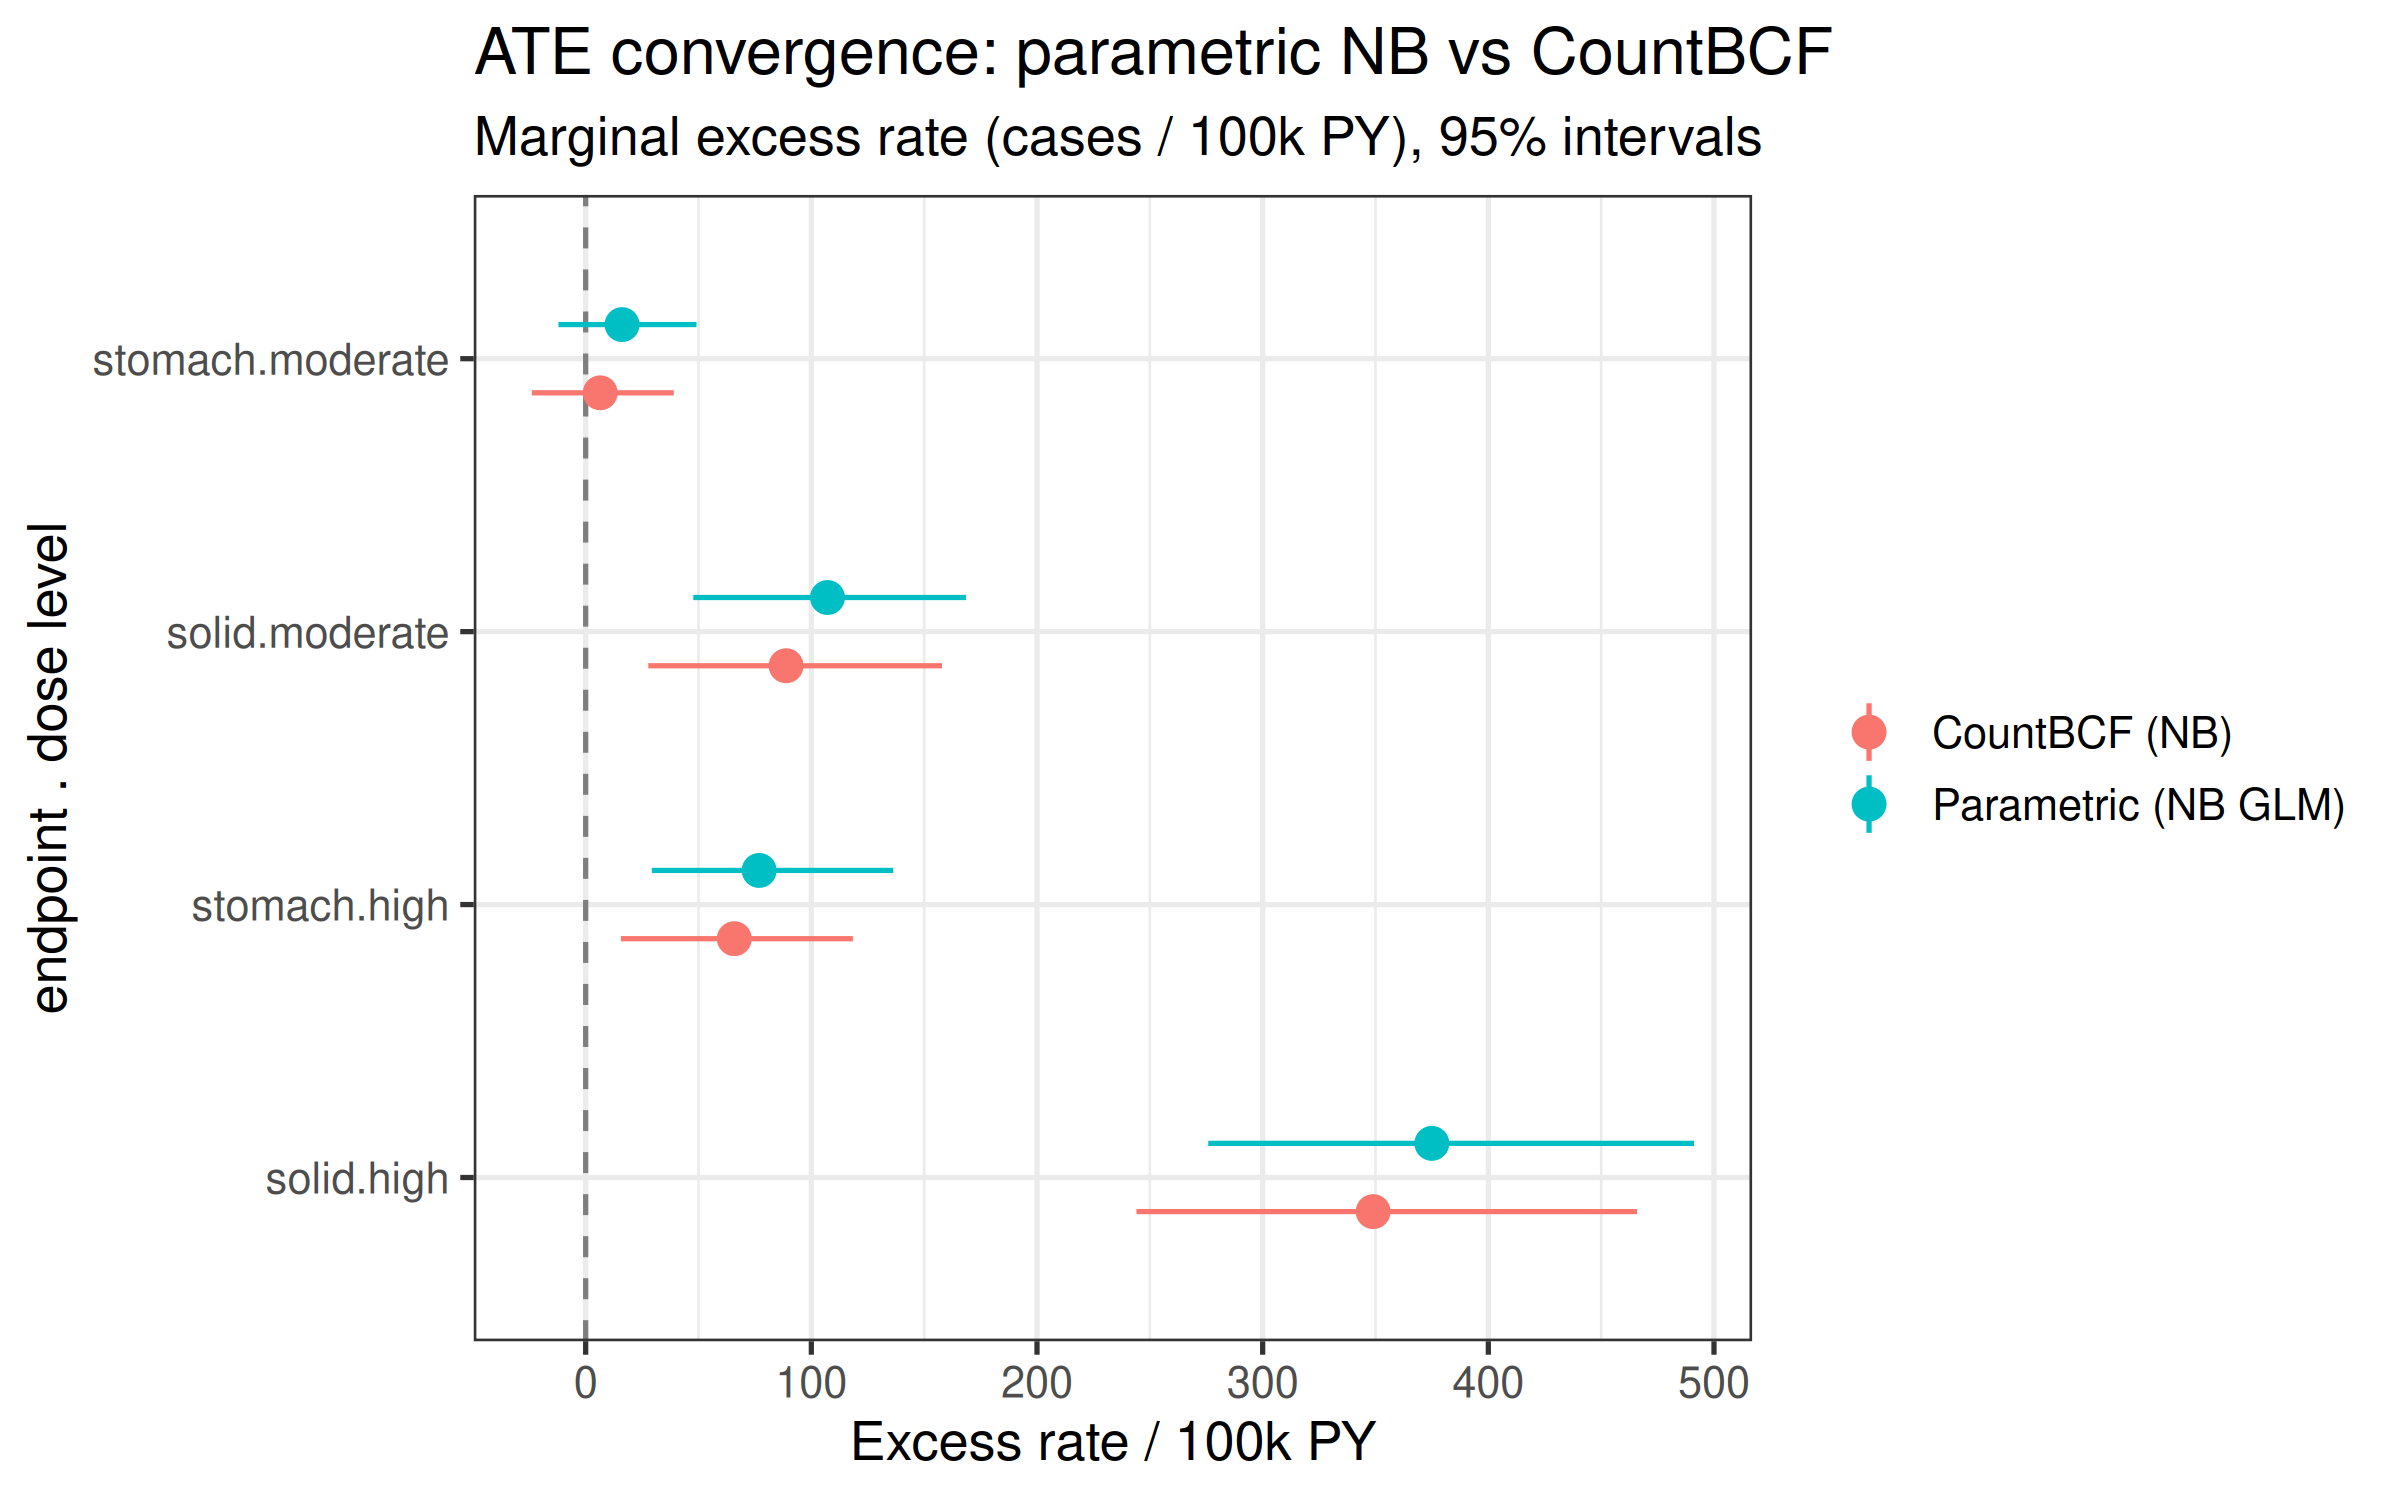
\includegraphics[width=0.78\textwidth]{ate_convergence.png}
\caption{ATE convergence on the absolute scale: CountBCF (NB) versus the
adjusted NB GLM, marginal excess rate (cases$/10^5$~PY) with $95\%$
intervals, for all four endpoint $\times$ dose-level contrasts. The two
estimators are nearly coincident on every contrast, with CountBCF
positioned a touch toward the null --- the expected signature of BCF's
regularization. The moderate-dose stomach contrast straddles zero for both
methods.}
\label{fig:ate-conv}
\end{figure}

The convergence is reassuring precisely because the parametric route is
fragile exactly where the paper argues it should be. Two illustrations from
the same data make the point. First, overdispersion inflates false
confidence: the minimal Poisson model is overdispersed (Pearson
$\chi^2/\text{df}\approx 3.6$ for both endpoints), and conditioning on
covariates only partly removes it, so naive Poisson intervals would be
spuriously narrow and NB is genuinely needed. Second, and more strikingly,
minimal NB models blow up in sparse cells: the minimal NB GLM for high-dose
stomach returns RR $=6.8$ with a $95\%$ interval of $[0.04,\,1119]$ ---
numerically useless --- while the minimal NB for moderate-dose solid
\emph{flips sign} relative to its Poisson counterpart. The parametric answer
depends on which GLM and which covariate set the analyst happens to choose.
CountBCF sidesteps this menu entirely: one model, stable across all four
contrasts, with the count likelihood and regularization handled internally.

The propensity specification supplies a concrete, teachable lesson that
validates the design choice of Section~\ref{sec:applied-design}. Distance from
the hypocentre is the \emph{assignment mechanism} for dose: it is
near-deterministic of the dose a survivor received and, under the standard LSS
assumption, affects cancer risk \emph{only through} that dose. It is therefore
a near-instrument, sitting off the confounding path rather than on it.
Conditioning on such a variable does two harmful things at once. First, it
\emph{collapses overlap} --- building the propensity from distance clamps the
estimated scores at $0$ and $1$, leaving no comparable treated and control
cells. Second, because an instrument lies off the confounding path,
conditioning on it does not remove confounding but \emph{amplifies} whatever
residual confounding remains. The high-dose solid estimate accordingly does
not merely widen; it flips to a biased RR $=0.57$ --- a sign reversal that is
the joint signature of both failures, not of a large variance alone. Building
the propensity from the \emph{demographic} confounders instead yields
well-overlapped scores ($\hat\pi\in[0.26,0.47]$, near-balanced across groups)
and the correct RR $=1.56$. A variable that determines treatment assignment
belongs in neither the propensity model nor the outcome forest when doing so
annihilates positivity; CountBCF's behaviour here is a clean demonstration of
the principle \citep{rosenbaum1983central}.

\subsection{Heterogeneity: the two master gradients}
\label{sec:applied-cate}

The ATE is a single number per contrast; CountBCF returns a full posterior
CATE for each of the $\sim$4\,660 solid (and $\sim$4\,602 stomach) cells in
the high-dose contrast. The heterogeneity is real and signed: for high-dose
solid cancer the per-cell CATE has median $346/10^5$~PY (IQR $[185,593]$,
range $[20,3339]$), with $100\%$ of cells positive and $68.8\%$ of cells'
$95\%$ credible intervals excluding zero; stomach has the same shape at about
one-fifth the magnitude ($55.0\%$ of intervals excluding zero). Radiation
raises the rate in every covariate profile, but the size of that increase
varies roughly $150$-fold across cells --- heterogeneity, not noise. With
\emph{no} interaction term specified, the BCF prior organises that
heterogeneity into the two textbook gradients of radiation epidemiology.

\textbf{Gradient 1 --- the relative excess falls steeply with age at
exposure.} The person-year-weighted ERR for high-dose solid cancer declines
nearly five-fold from $\approx 1.23$ for those exposed before age $10$ to
$\approx 0.25$ for those exposed after age $40$
(Table~\ref{tab:applied-gradients} and Figure~\ref{fig:err-agex}). This is
the single most robust qualitative finding in the LSS literature, recovered
here nonparametrically. The fitted smooths also expose a nuance a coarse
summary would flatten: the decline \emph{plateaus} around age-at-exposure
$40$--$50$ at $\approx 0.24$--$0.25$ rather than continuing toward zero, with
a faint upturn at the oldest (and sparsest) exposure ages --- both visible in
Figure~\ref{fig:err-agex}, and a feature we return to in
Section~\ref{sec:applied-divergence}. The two sex curves are nearly
superimposed for the solid aggregate but cleanly separated (female above
male) for stomach, foreshadowing Section~\ref{sec:applied-divergence}.

\begin{figure}[htbp]
\centering
\begin{subfigure}{0.49\textwidth}
  \centering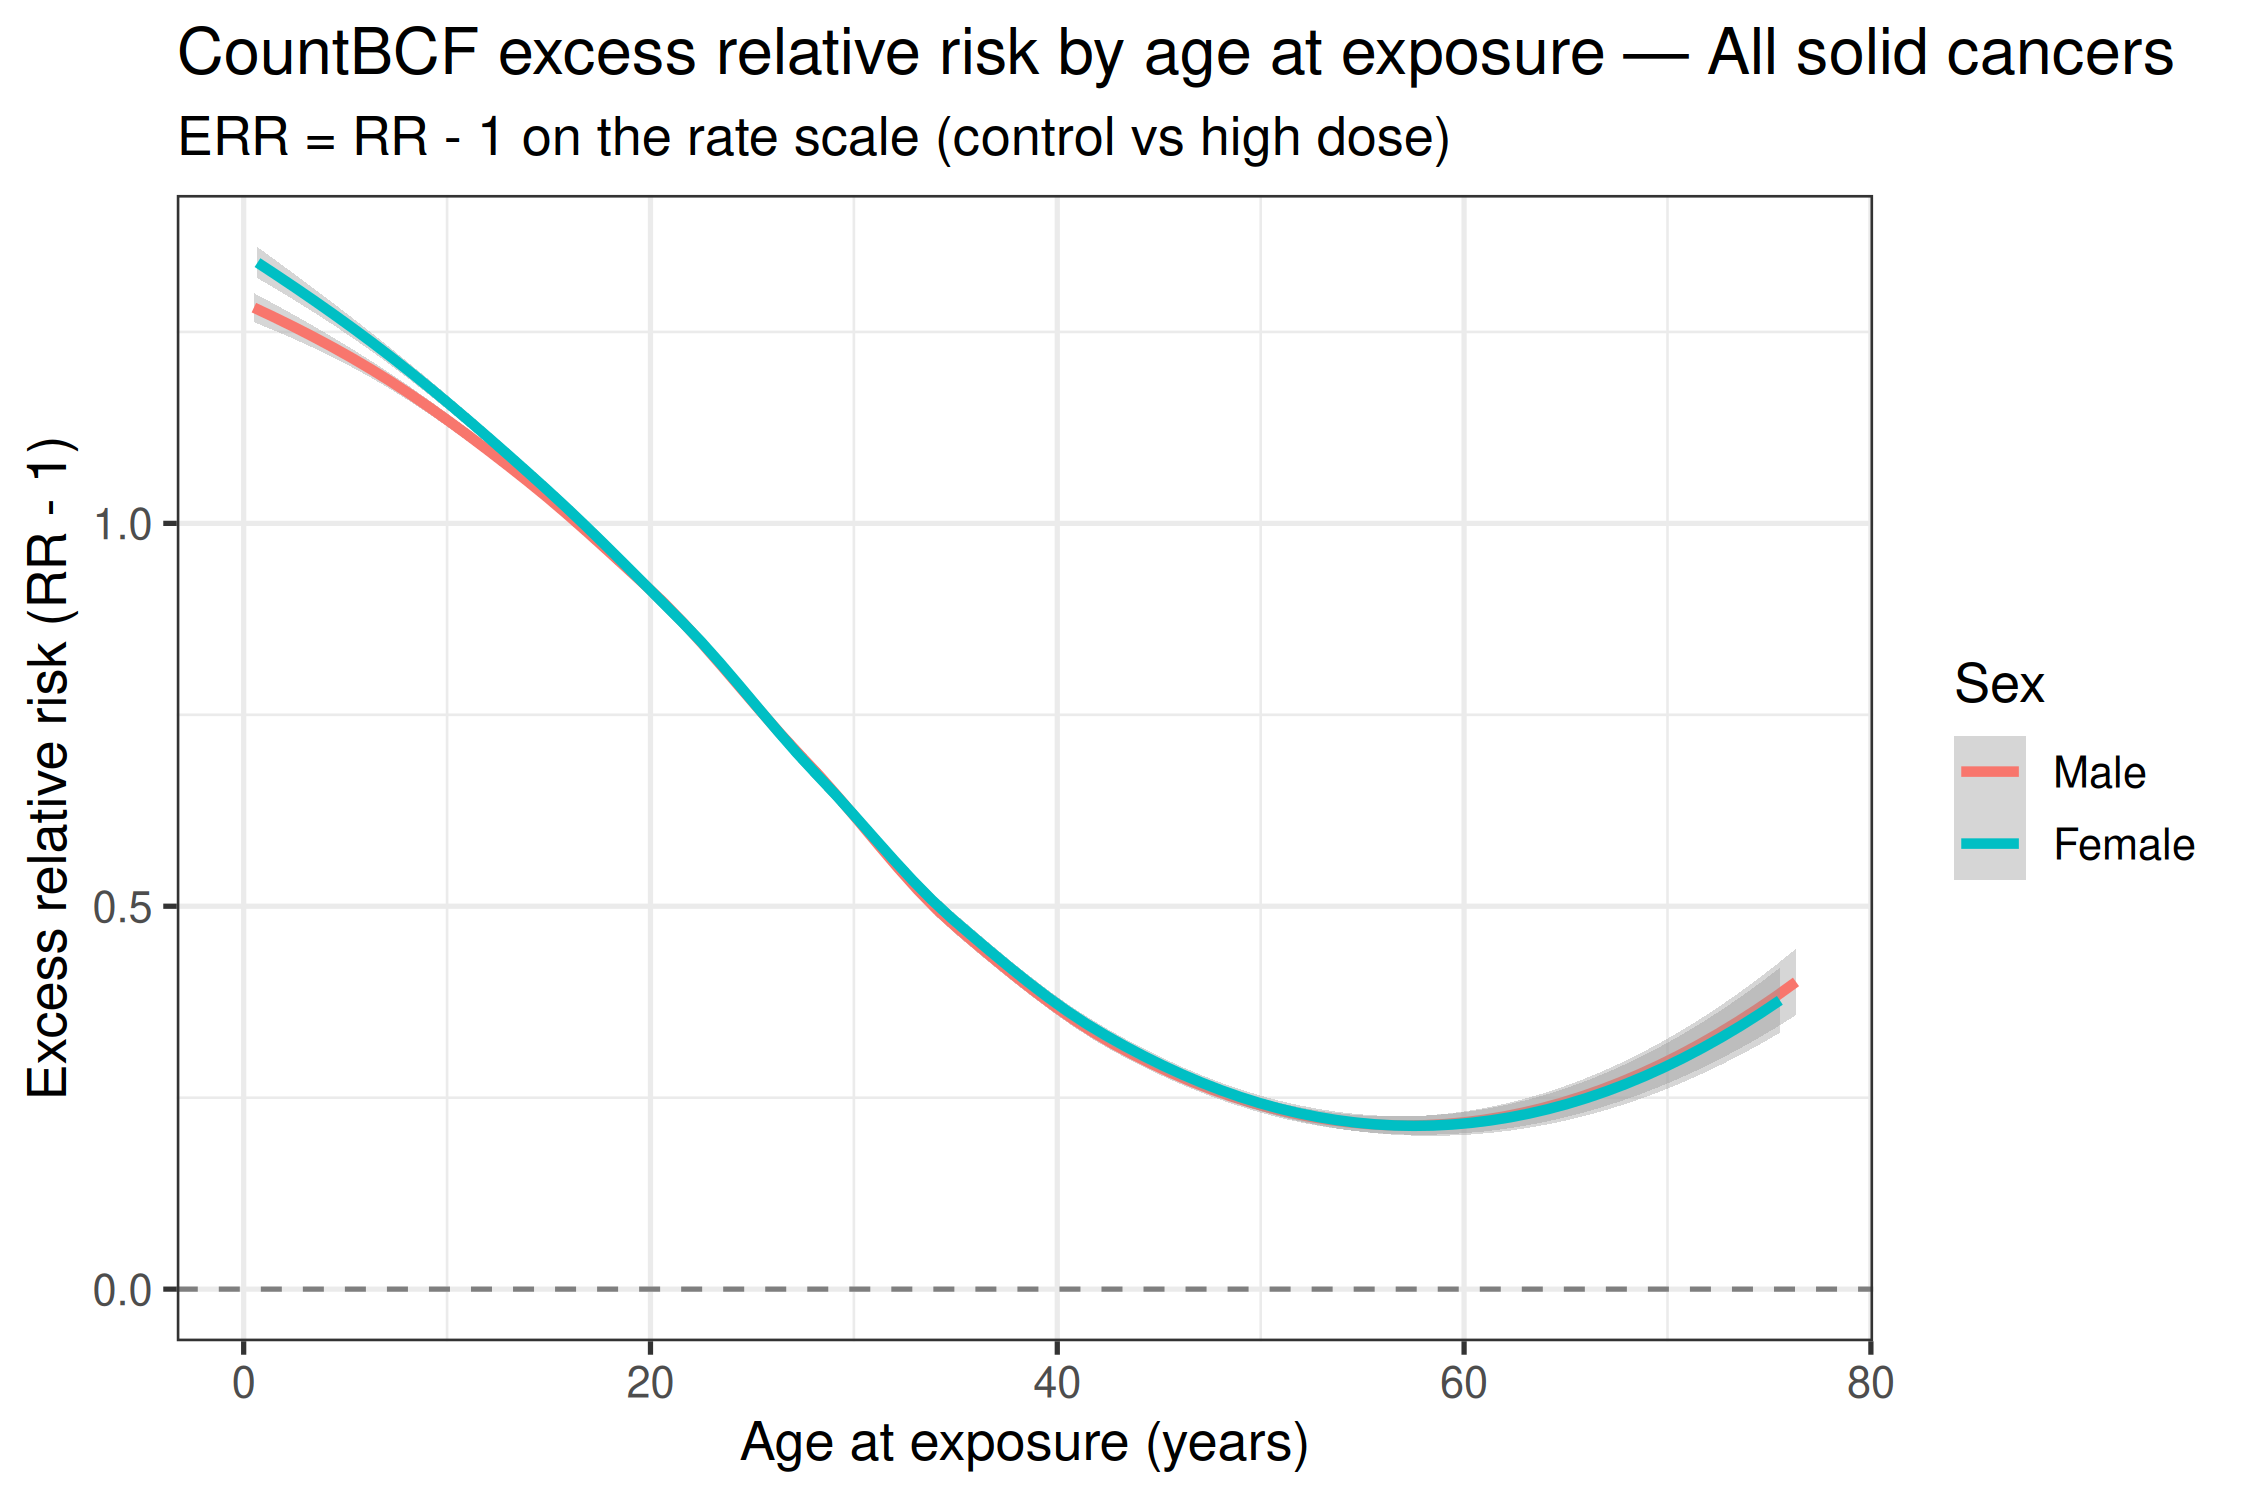
\includegraphics[width=\linewidth]{solid_err_by_agex_sex.png}
  \caption{All solid cancers}\label{fig:err-agex-solid}
\end{subfigure}
\hfill
\begin{subfigure}{0.49\textwidth}
  \centering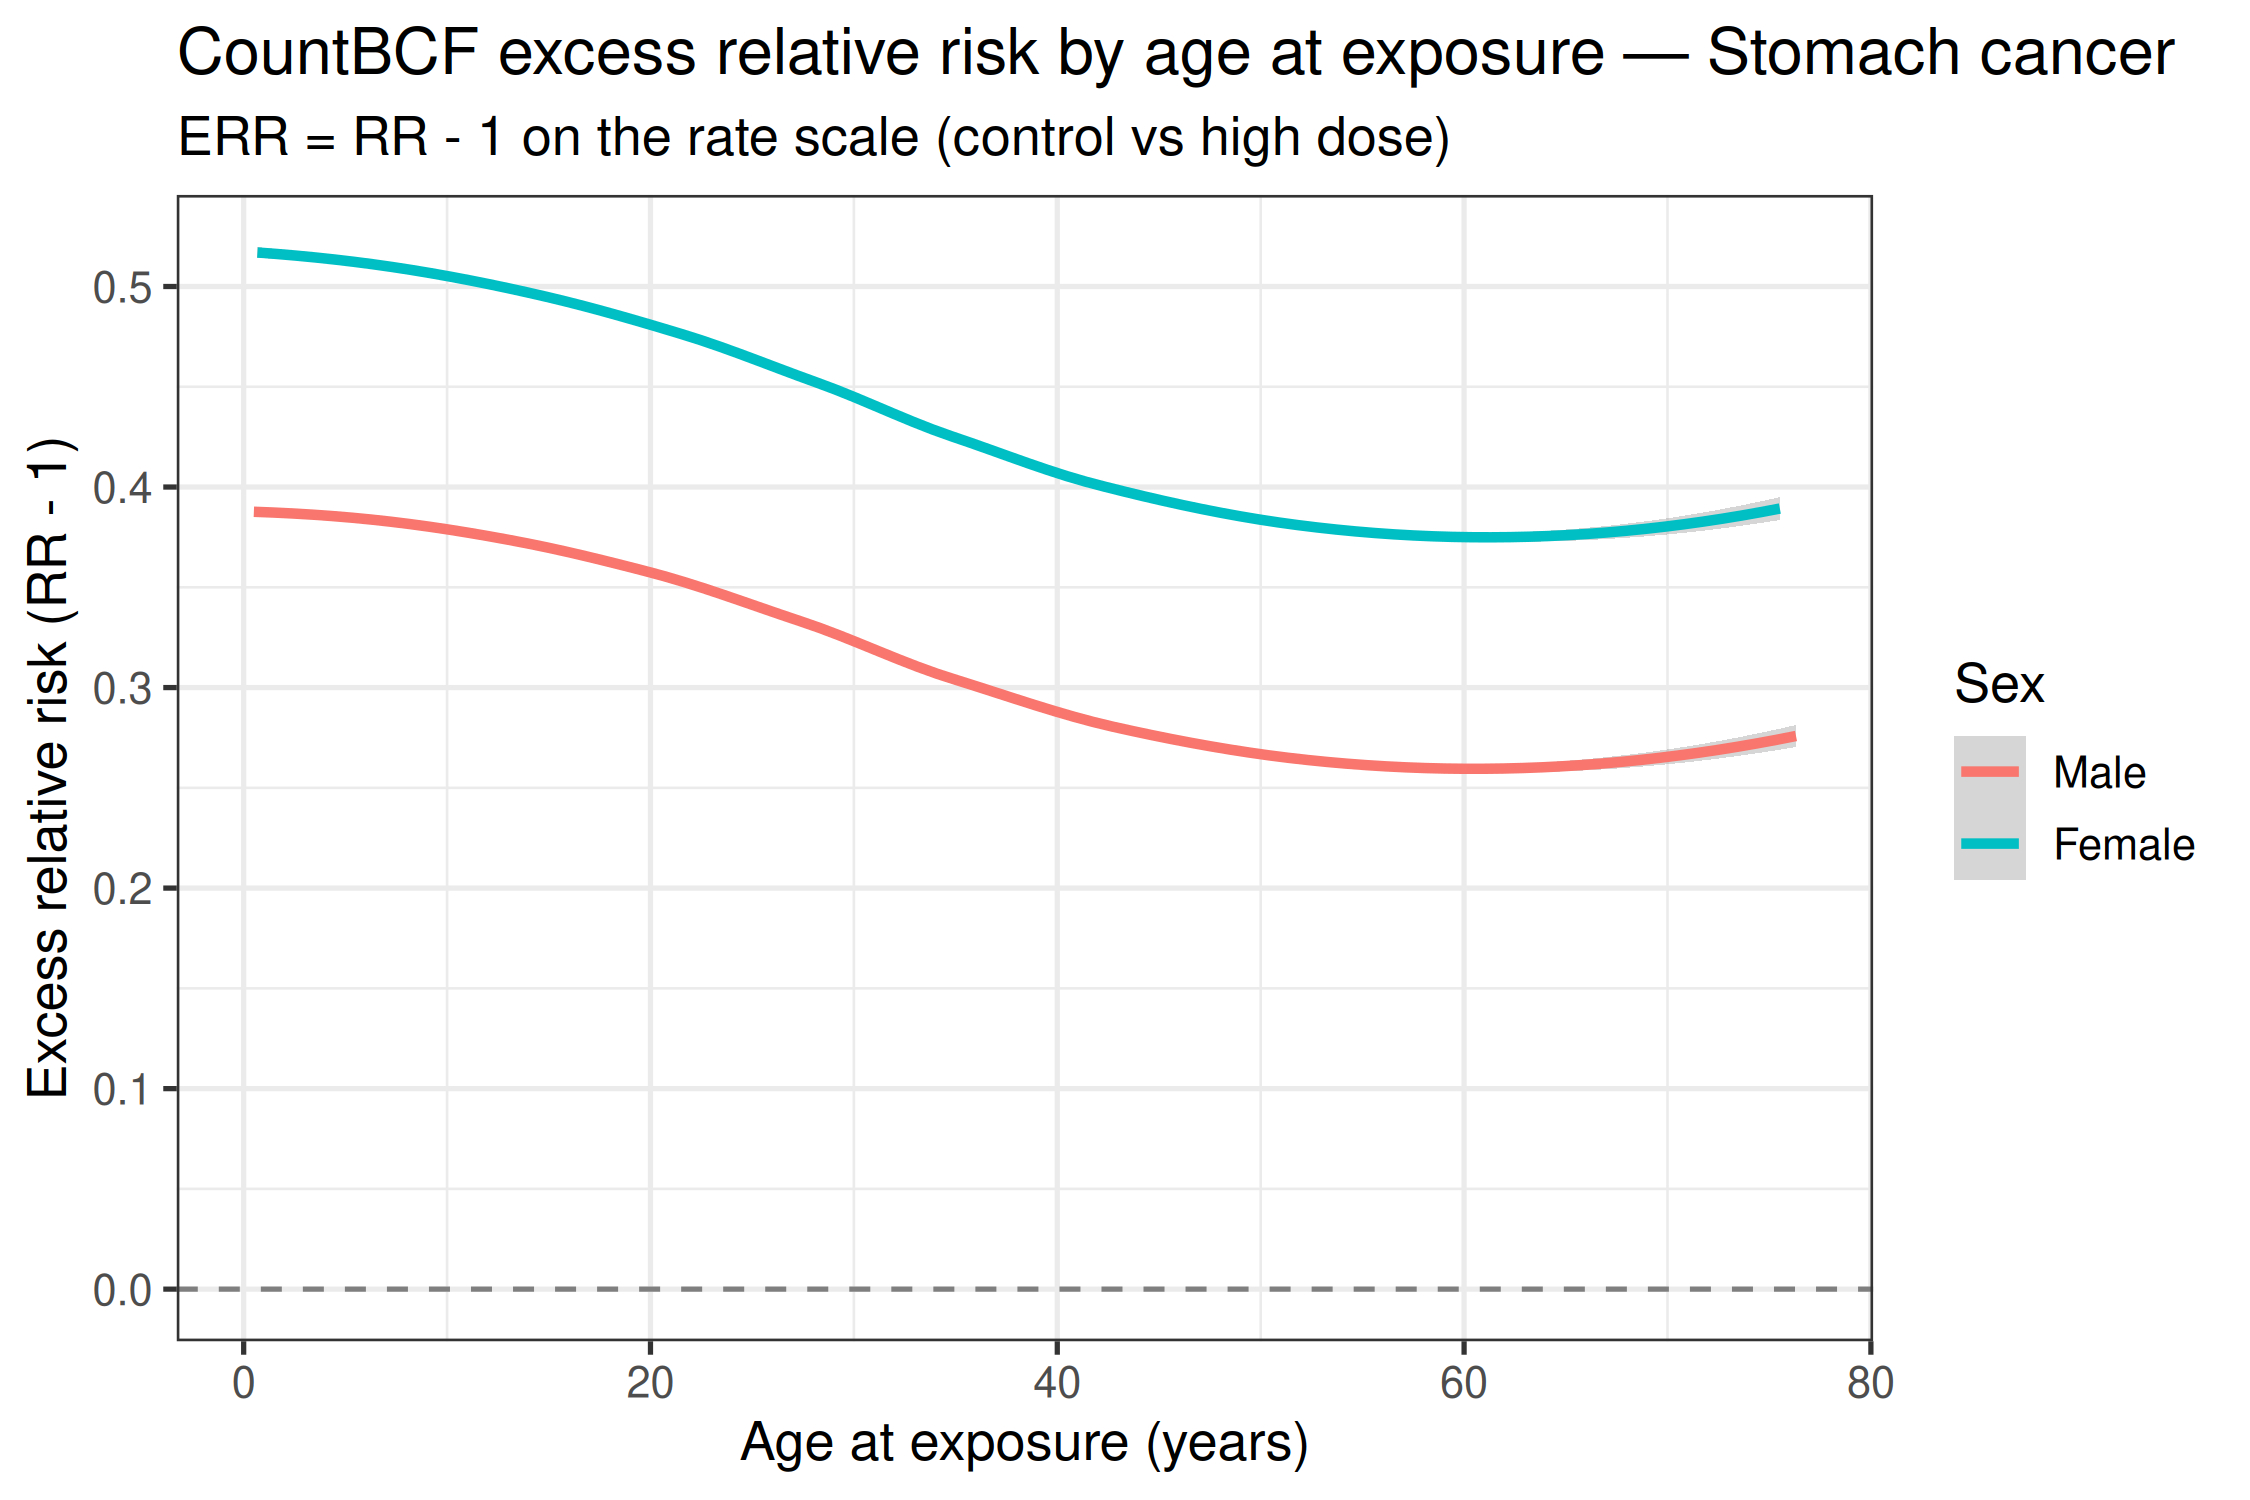
\includegraphics[width=\linewidth]{stomach_err_by_agex_sex.png}
  \caption{Stomach}\label{fig:err-agex-stomach}
\end{subfigure}
\caption{\textbf{Gradient 1 (multiplicative scale).} CountBCF excess relative
risk (ERR $=$ RR $-1$) for the high-dose contrast as a function of age at
exposure, by sex (smooths with $95\%$ bands over per-cell posterior means).
Solid-cancer ERR falls steeply with older exposure age, then plateaus near
$0.25$ around age $50$ with a faint upturn at the oldest, sparsest exposure
ages (Section~\ref{sec:applied-divergence}). The stomach slope is far
shallower. Sex curves are near-coincident for solid but female-above-male for
stomach.}
\label{fig:err-agex}
\end{figure}

\textbf{Gradient 2 --- the absolute excess rises with attained age.} On the
absolute scale the EAR climbs roughly seven-fold (solid) and fifteen-fold
(stomach) across the attained-age range
(Table~\ref{tab:applied-gradients}, right block, and
Figure~\ref{fig:ear-age}), because EAR $\approx$ baseline incidence $\times$
ERR and baseline solid-cancer incidence rises steeply with age; males carry
the larger absolute excess throughout (Figure~\ref{fig:ear-age}, red smooth
above teal). The two gradients are not contradictory: they are the
multiplicative and additive projections of one effect surface, and CountBCF
renders both from a single fit.

\begin{figure}[htbp]
\centering
\begin{subfigure}{0.49\textwidth}
  \centering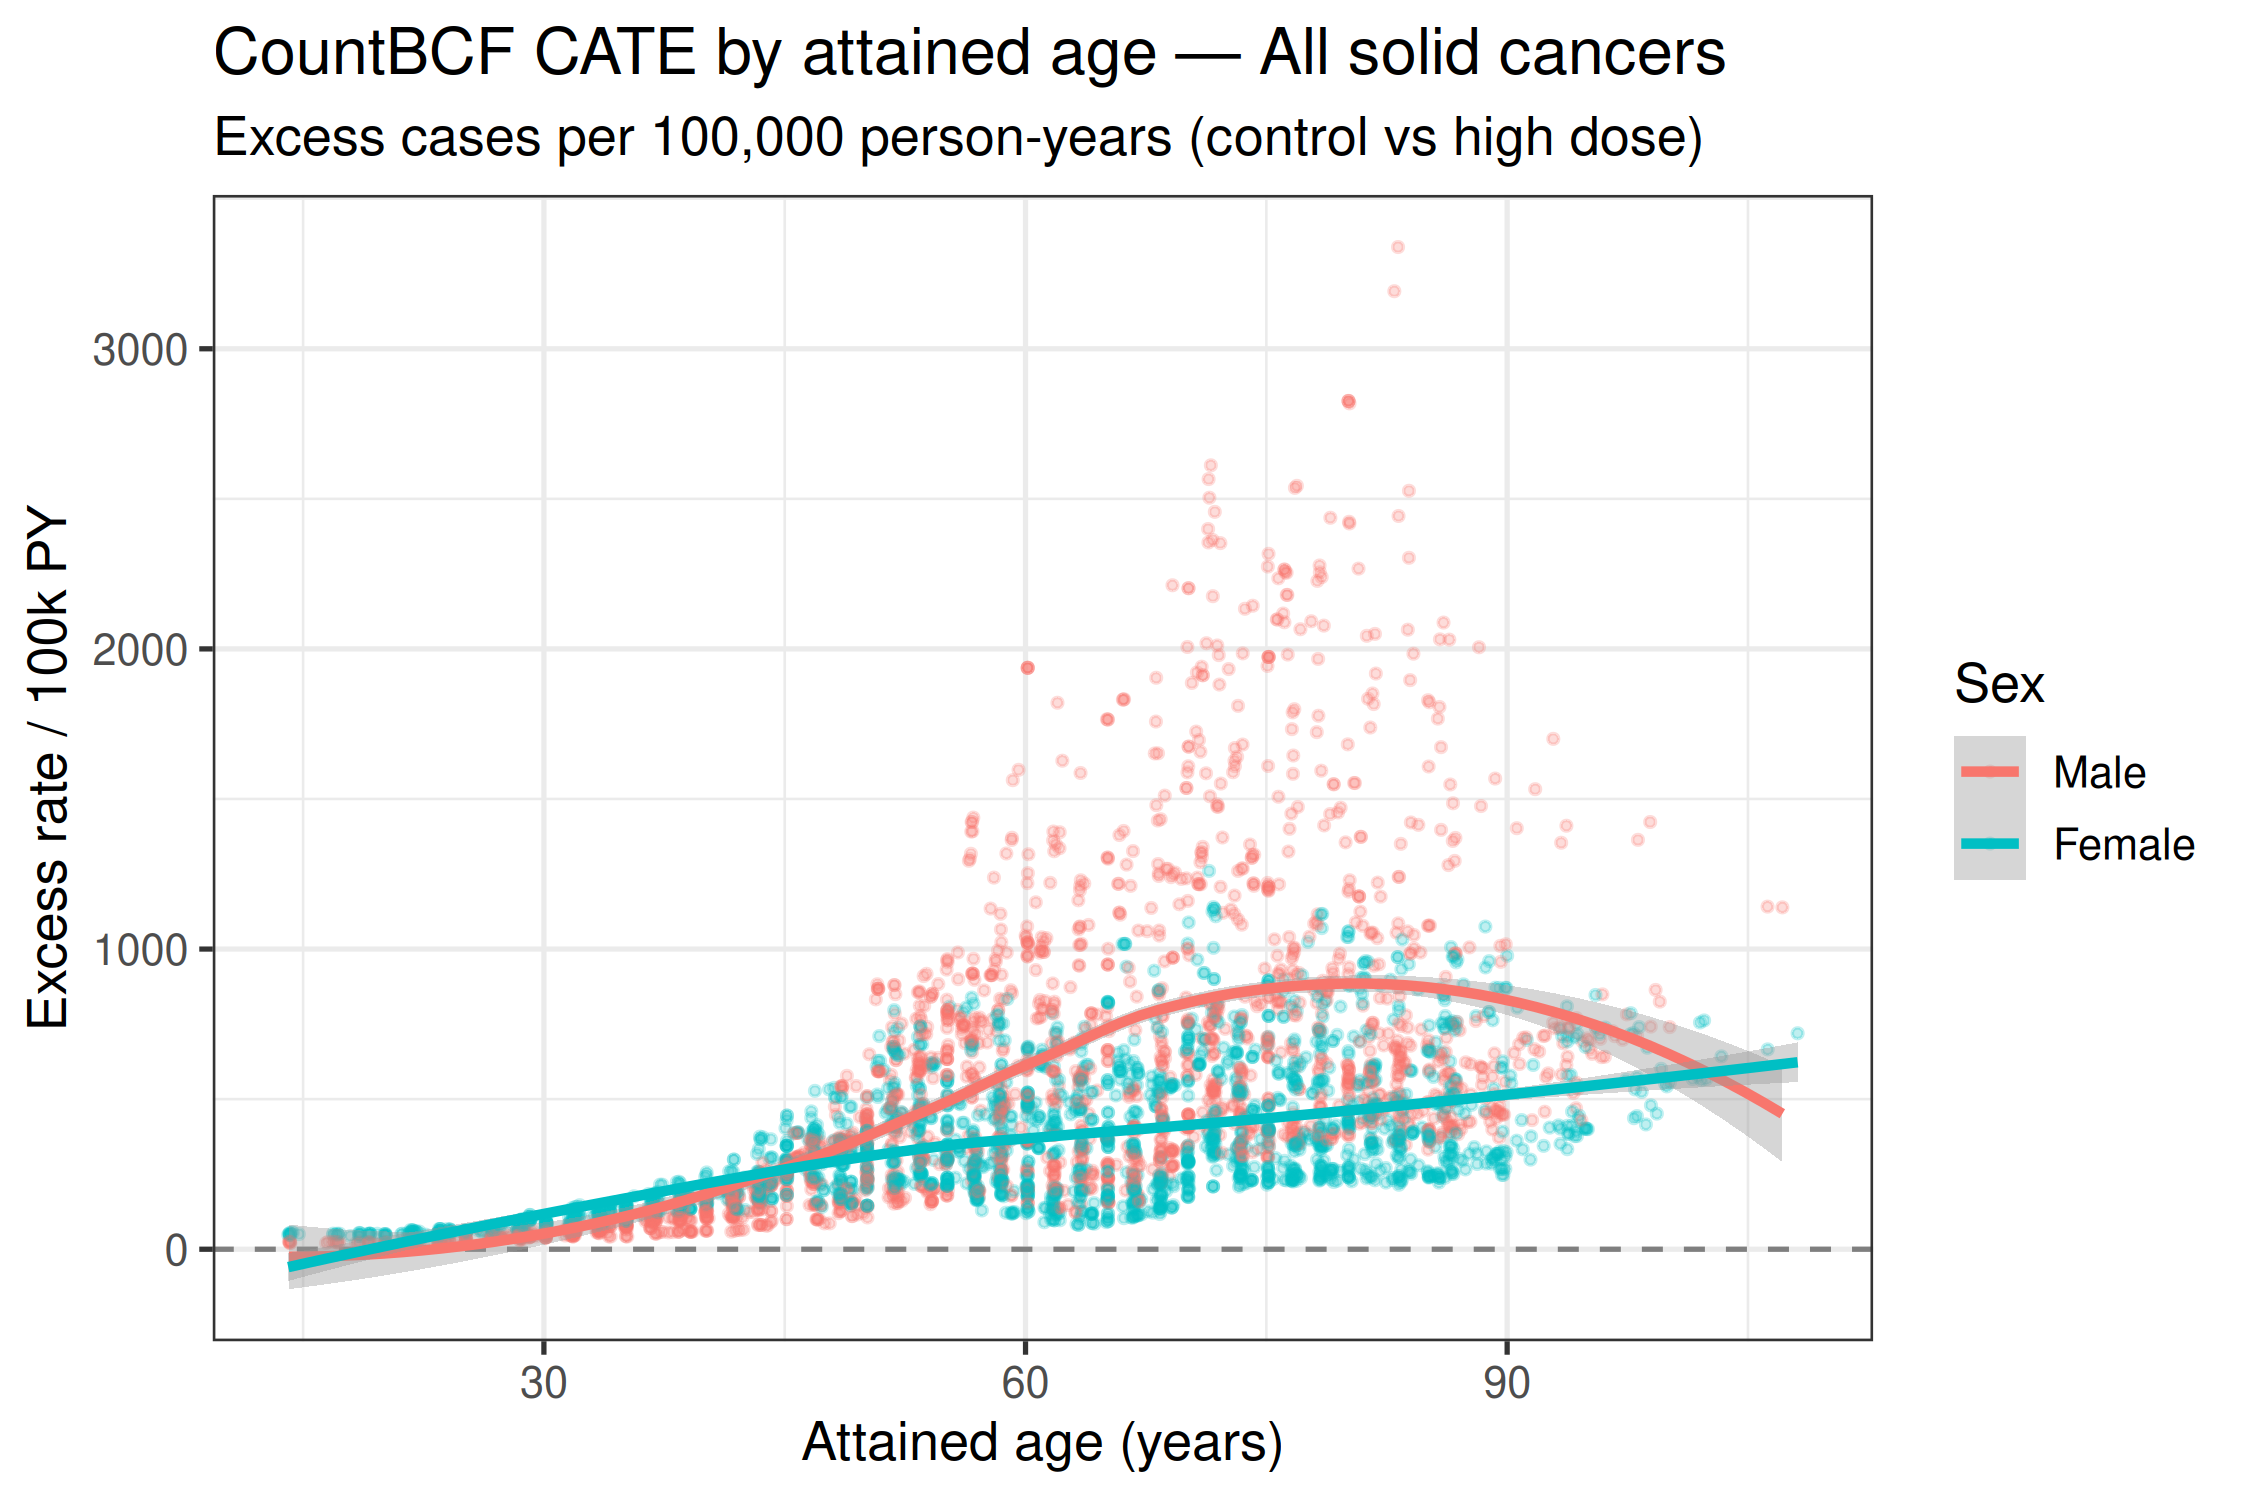
\includegraphics[width=\linewidth]{solid_cate_by_age_sex.png}
  \caption{All solid cancers}\label{fig:ear-age-solid}
\end{subfigure}
\hfill
\begin{subfigure}{0.49\textwidth}
  \centering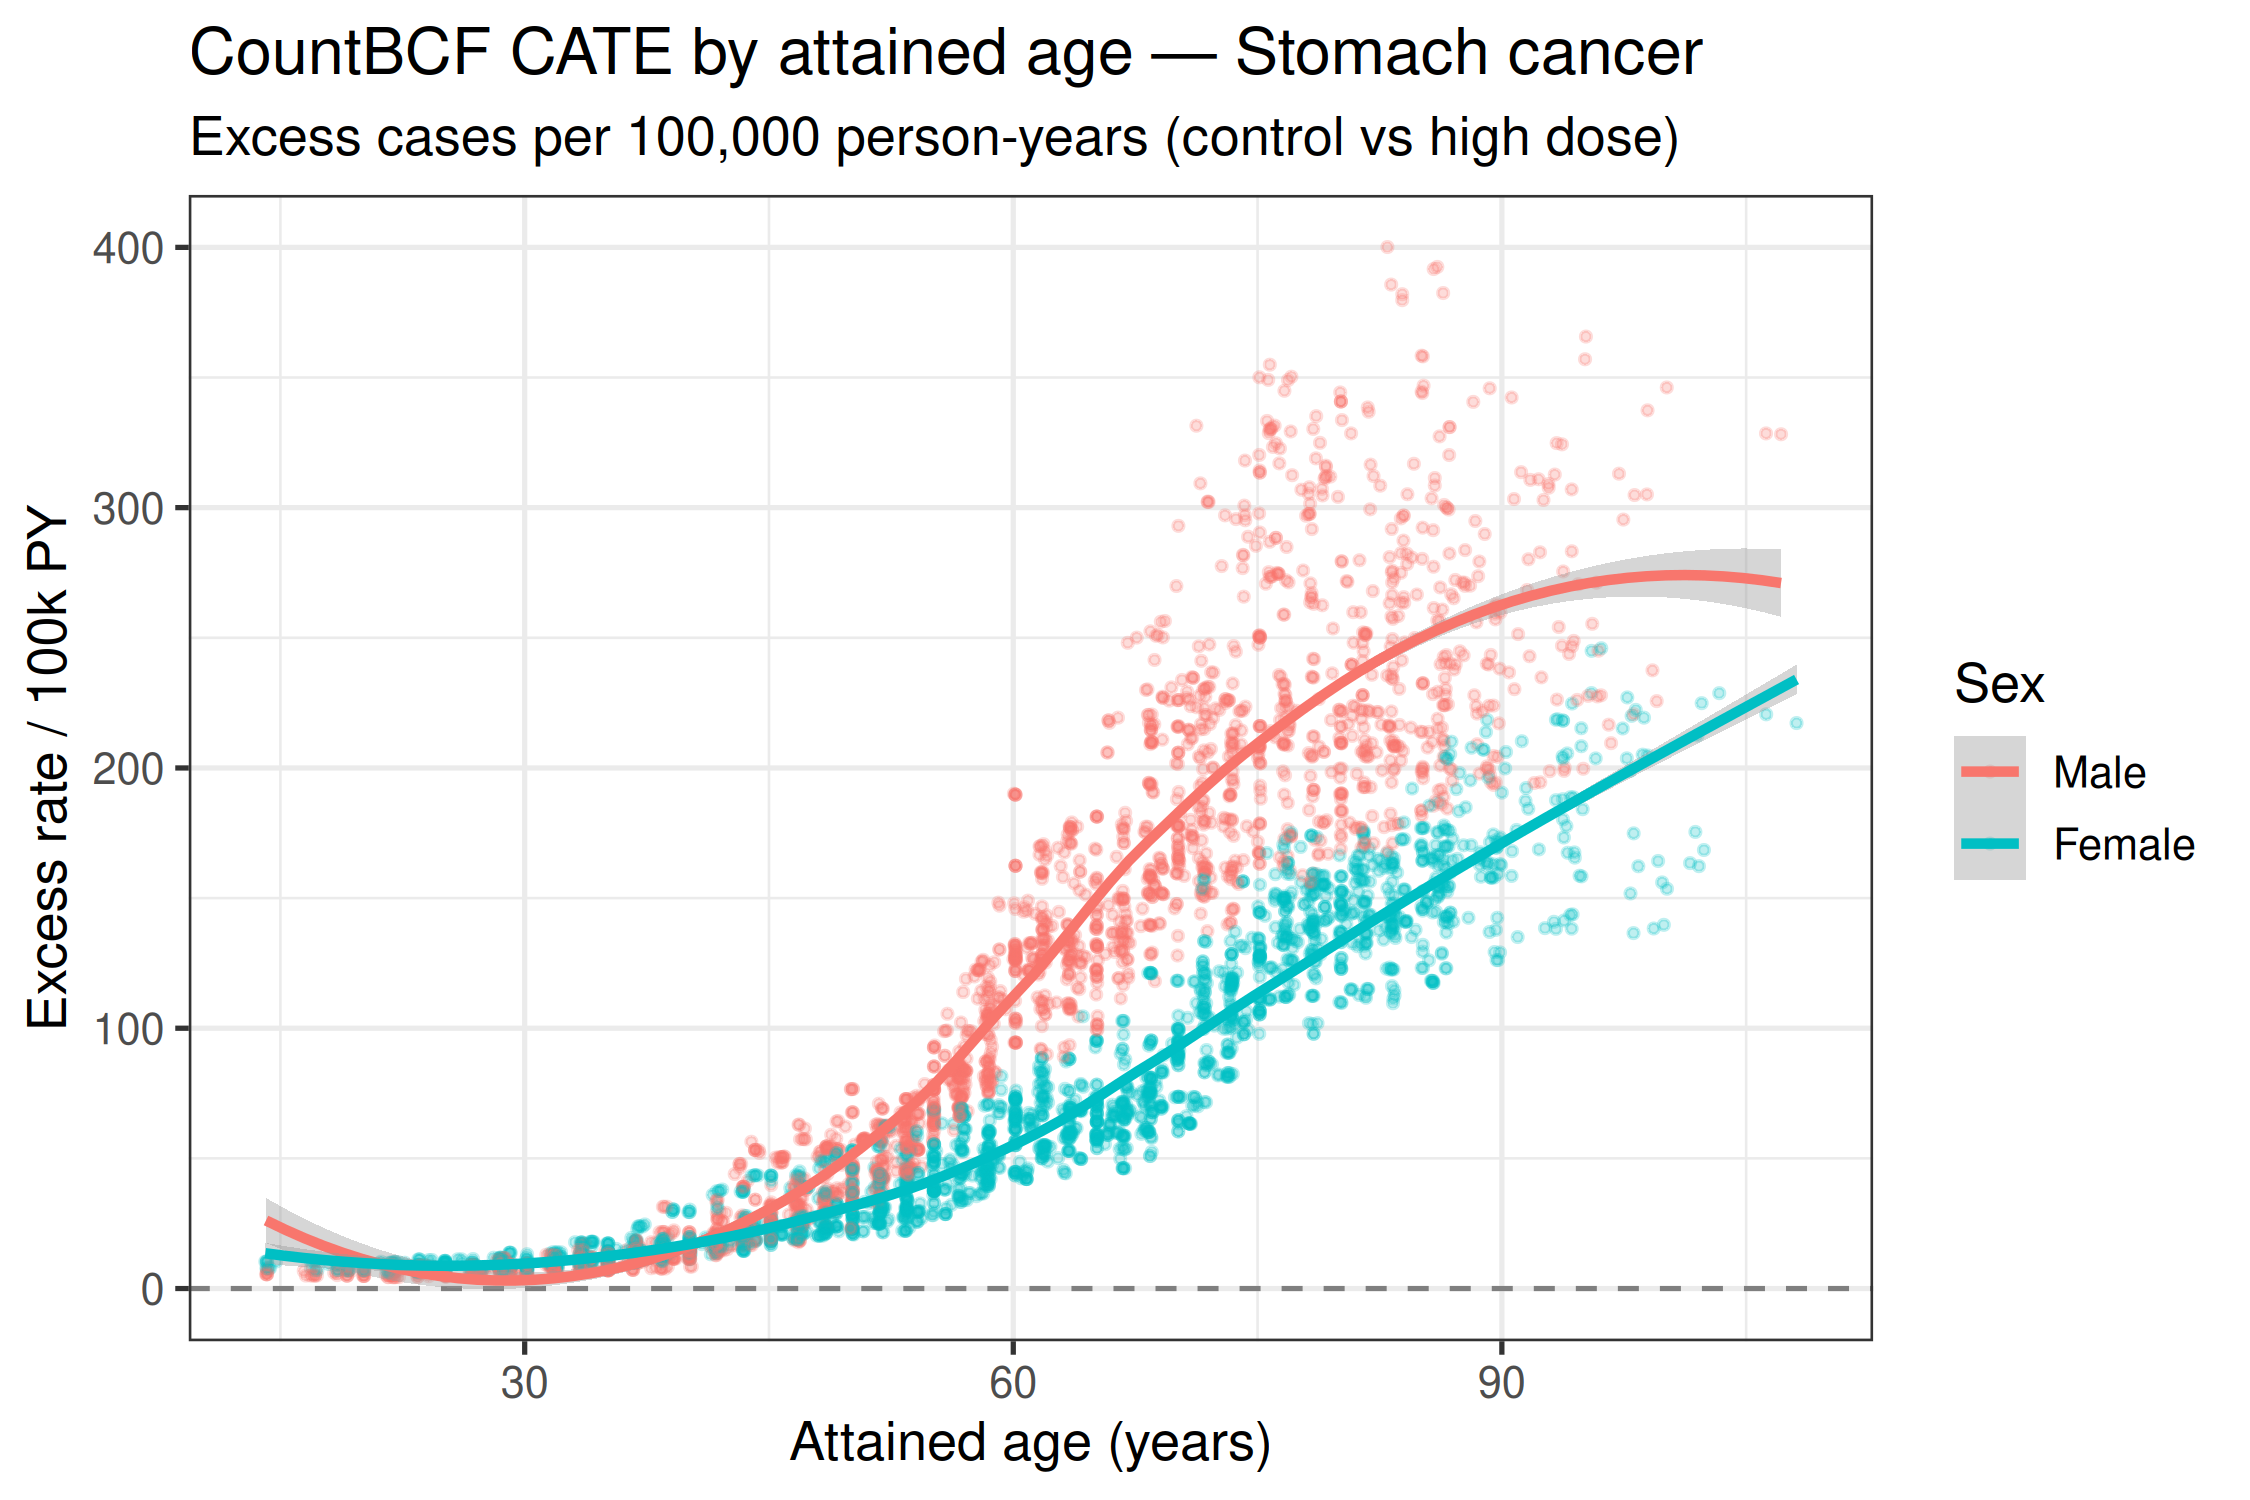
\includegraphics[width=\linewidth]{stomach_cate_by_age_sex.png}
  \caption{Stomach}\label{fig:ear-age-stomach}
\end{subfigure}
\caption{\textbf{Gradient 2 (absolute scale).} Per-cell CATE (excess
cases$/10^5$~PY) for the high-dose contrast against attained age, by sex
(points are individual cells; lines are sex-specific smooths). The absolute
excess rises with attained age as the baseline incidence climbs, even as the
relative multiplier of Figure~\ref{fig:err-agex} fades; the male smooth sits
above the female throughout.}
\label{fig:ear-age}
\end{figure}

\begin{table}[htbp]
\centering
\caption{The two master gradients for the high-dose contrast,
person-year-weighted. Left: ERR (and EAR) by age at exposure, with the mean
attained age at which each exposure-age band is observed. Right: EAR by
attained age. Note the EAR \emph{peak} at age-at-exposure 20--30 even though
ERR peaks at the youngest --- the classic EAR-vs-ERR tension
(Section~\ref{sec:applied-cate}).}
\label{tab:applied-gradients}
\small
\begin{tabular}{lccc@{\hskip 1.2cm}lcc}
\toprule
\multicolumn{4}{c}{By age at exposure (solid)} & \multicolumn{3}{c}{By attained age} \\
\cmidrule(r){1-4}\cmidrule(l){5-7}
Age at exp. & ERR & EAR$/10^5$ & mean att.\ age & Attained age & EAR solid & EAR stom. \\
\midrule
$<10$  & 1.232 & 261 & 37 & $<40$   & 86.3  & 10.4 \\
10--20 & 1.091 & 359 & 46 & 40--55  & 330.1 & 33.1 \\
20--30 & 0.793 & \textbf{422} & 55 & 55--70 & 458.6 & 88.8 \\
30--40 & 0.488 & 388 & 64 & 70+     & 584.7 & 155.3 \\
40--50 & 0.276 & 350 & 71 &         &       &      \\
50--60 & 0.244 & 349 & 76 &         &       &      \\
60+    & 0.246 & 340 & 82 &         &       &      \\
\bottomrule
\end{tabular}
\end{table}

The interplay of the two gradients surfaces a subtlety that neither shows
alone. The \emph{absolute} excess peaks for those exposed at $20$--$30$, not
for the youngest, even though the youngest carry by far the highest
\emph{relative} risk (Table~\ref{tab:applied-gradients}); plotting the
absolute excess against age at exposure (Figure~\ref{fig:ear-agex}) makes the
intermediate peak visible directly, in contrast to the monotone relative-scale
decline of Figure~\ref{fig:err-agex}. The driver is the cross-sectional
structure of the person-year table: each exposure-age band is observed over a
different attained-age window (rightmost column of
Table~\ref{tab:applied-gradients}), so the youngest-exposed are seen young, at
low baseline, and the $20$--$30$ band is seen at mean attained age $55$, where
the higher baseline more than compensates for the lower ERR. This is the
textbook EAR-vs-ERR tension \citep{pierce2000}, and CountBCF surfaces it
automatically: report ERR if you care about radiosensitivity, EAR if you care
about attributable burden --- they rank the exposure-age groups differently.
The resolution of the tension is the full two-dimensional effect surface
(Figure~\ref{fig:heatmap}): the excess concentrates toward old attained age
and younger-to-middle age at exposure --- the joint maximum of the
``long-fuse'' relative effect and the high absolute baseline --- and it is
this surface, not its one-dimensional margins, that is the deconfounded causal
object. Two further patterns complete the picture and are reported in full in
the supplementary analysis. Across time since exposure the solid ERR is
essentially flat ($\approx 0.80$) while the EAR rises about six-fold
($147\to905/10^5$~PY), i.e.\ the absolute excess grows through follow-up
because the baseline grows, not because the relative effect intensifies --- a
persistent multiplicative excess. And the heterogeneity scales coherently with
dose: the moderate-dose solid ERR runs $\approx 0.19$ (young) to $\approx
0.08$ (old), the same downward shape as high dose but compressed toward zero,
while moderate-dose stomach is a coherent null (RR $1.04$) --- a partial
negative control the model passes, inventing no heterogeneity where the dose
signal is weak.

\begin{figure}[htbp]
\centering
\begin{subfigure}{0.49\textwidth}
  \centering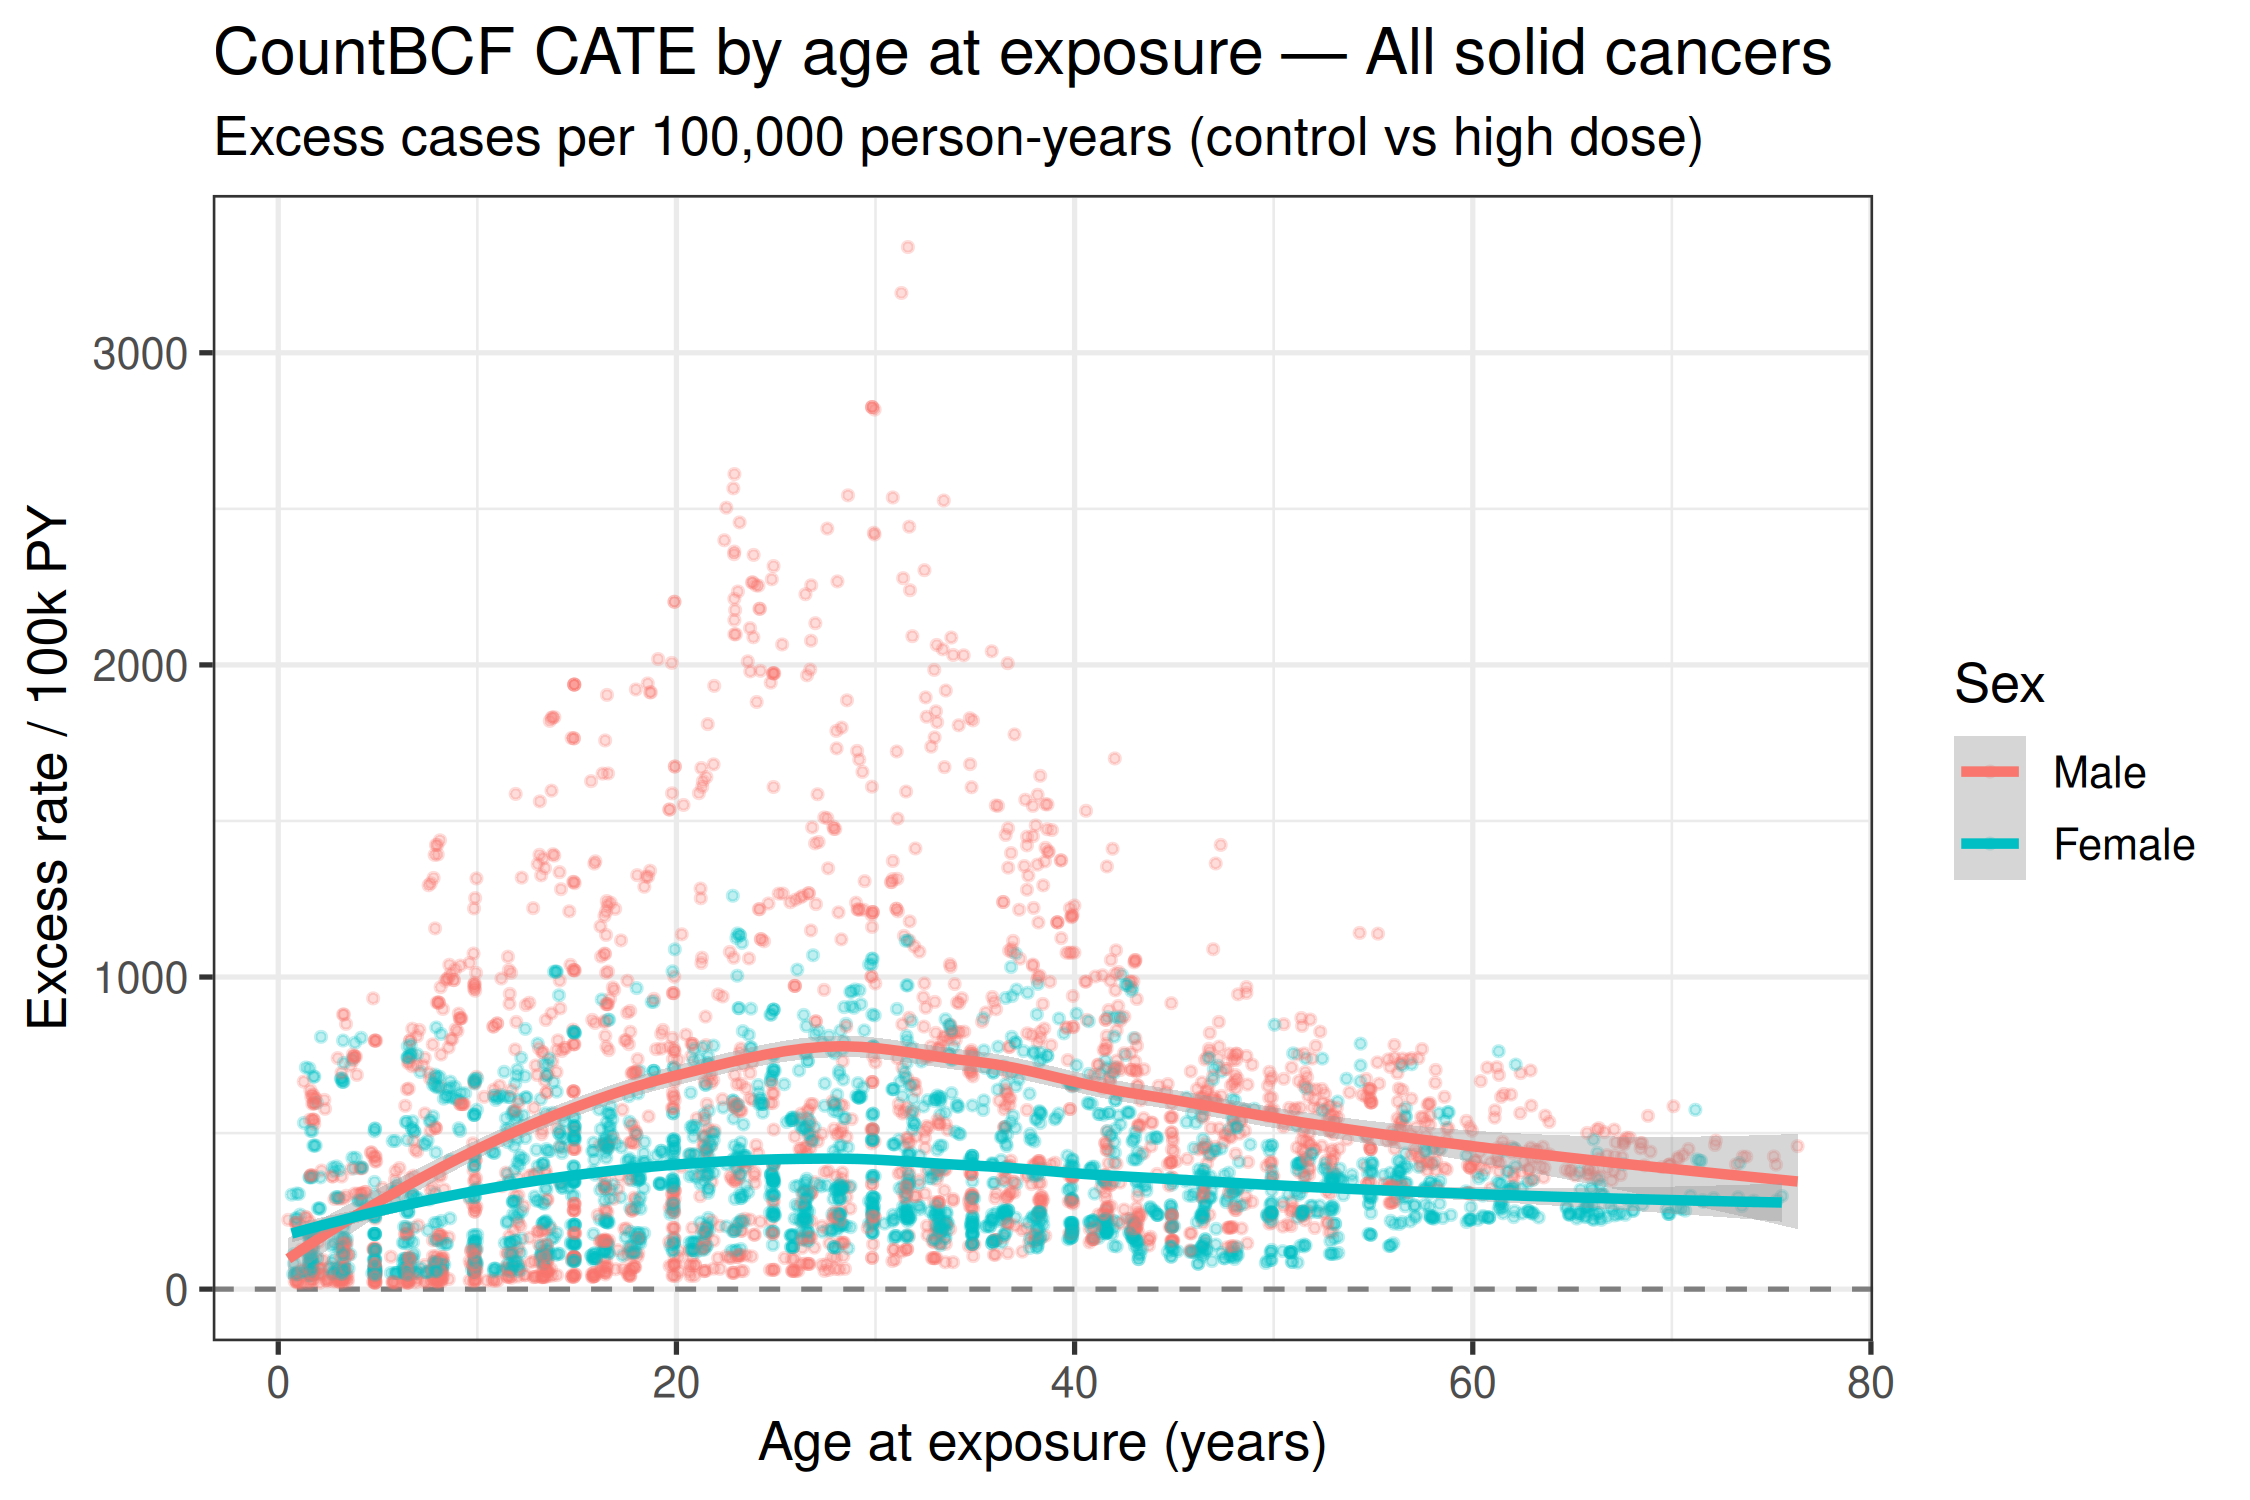
\includegraphics[width=\linewidth]{solid_cate_by_agex_sex.png}
  \caption{All solid cancers}\label{fig:ear-agex-solid}
\end{subfigure}
\hfill
\begin{subfigure}{0.49\textwidth}
  \centering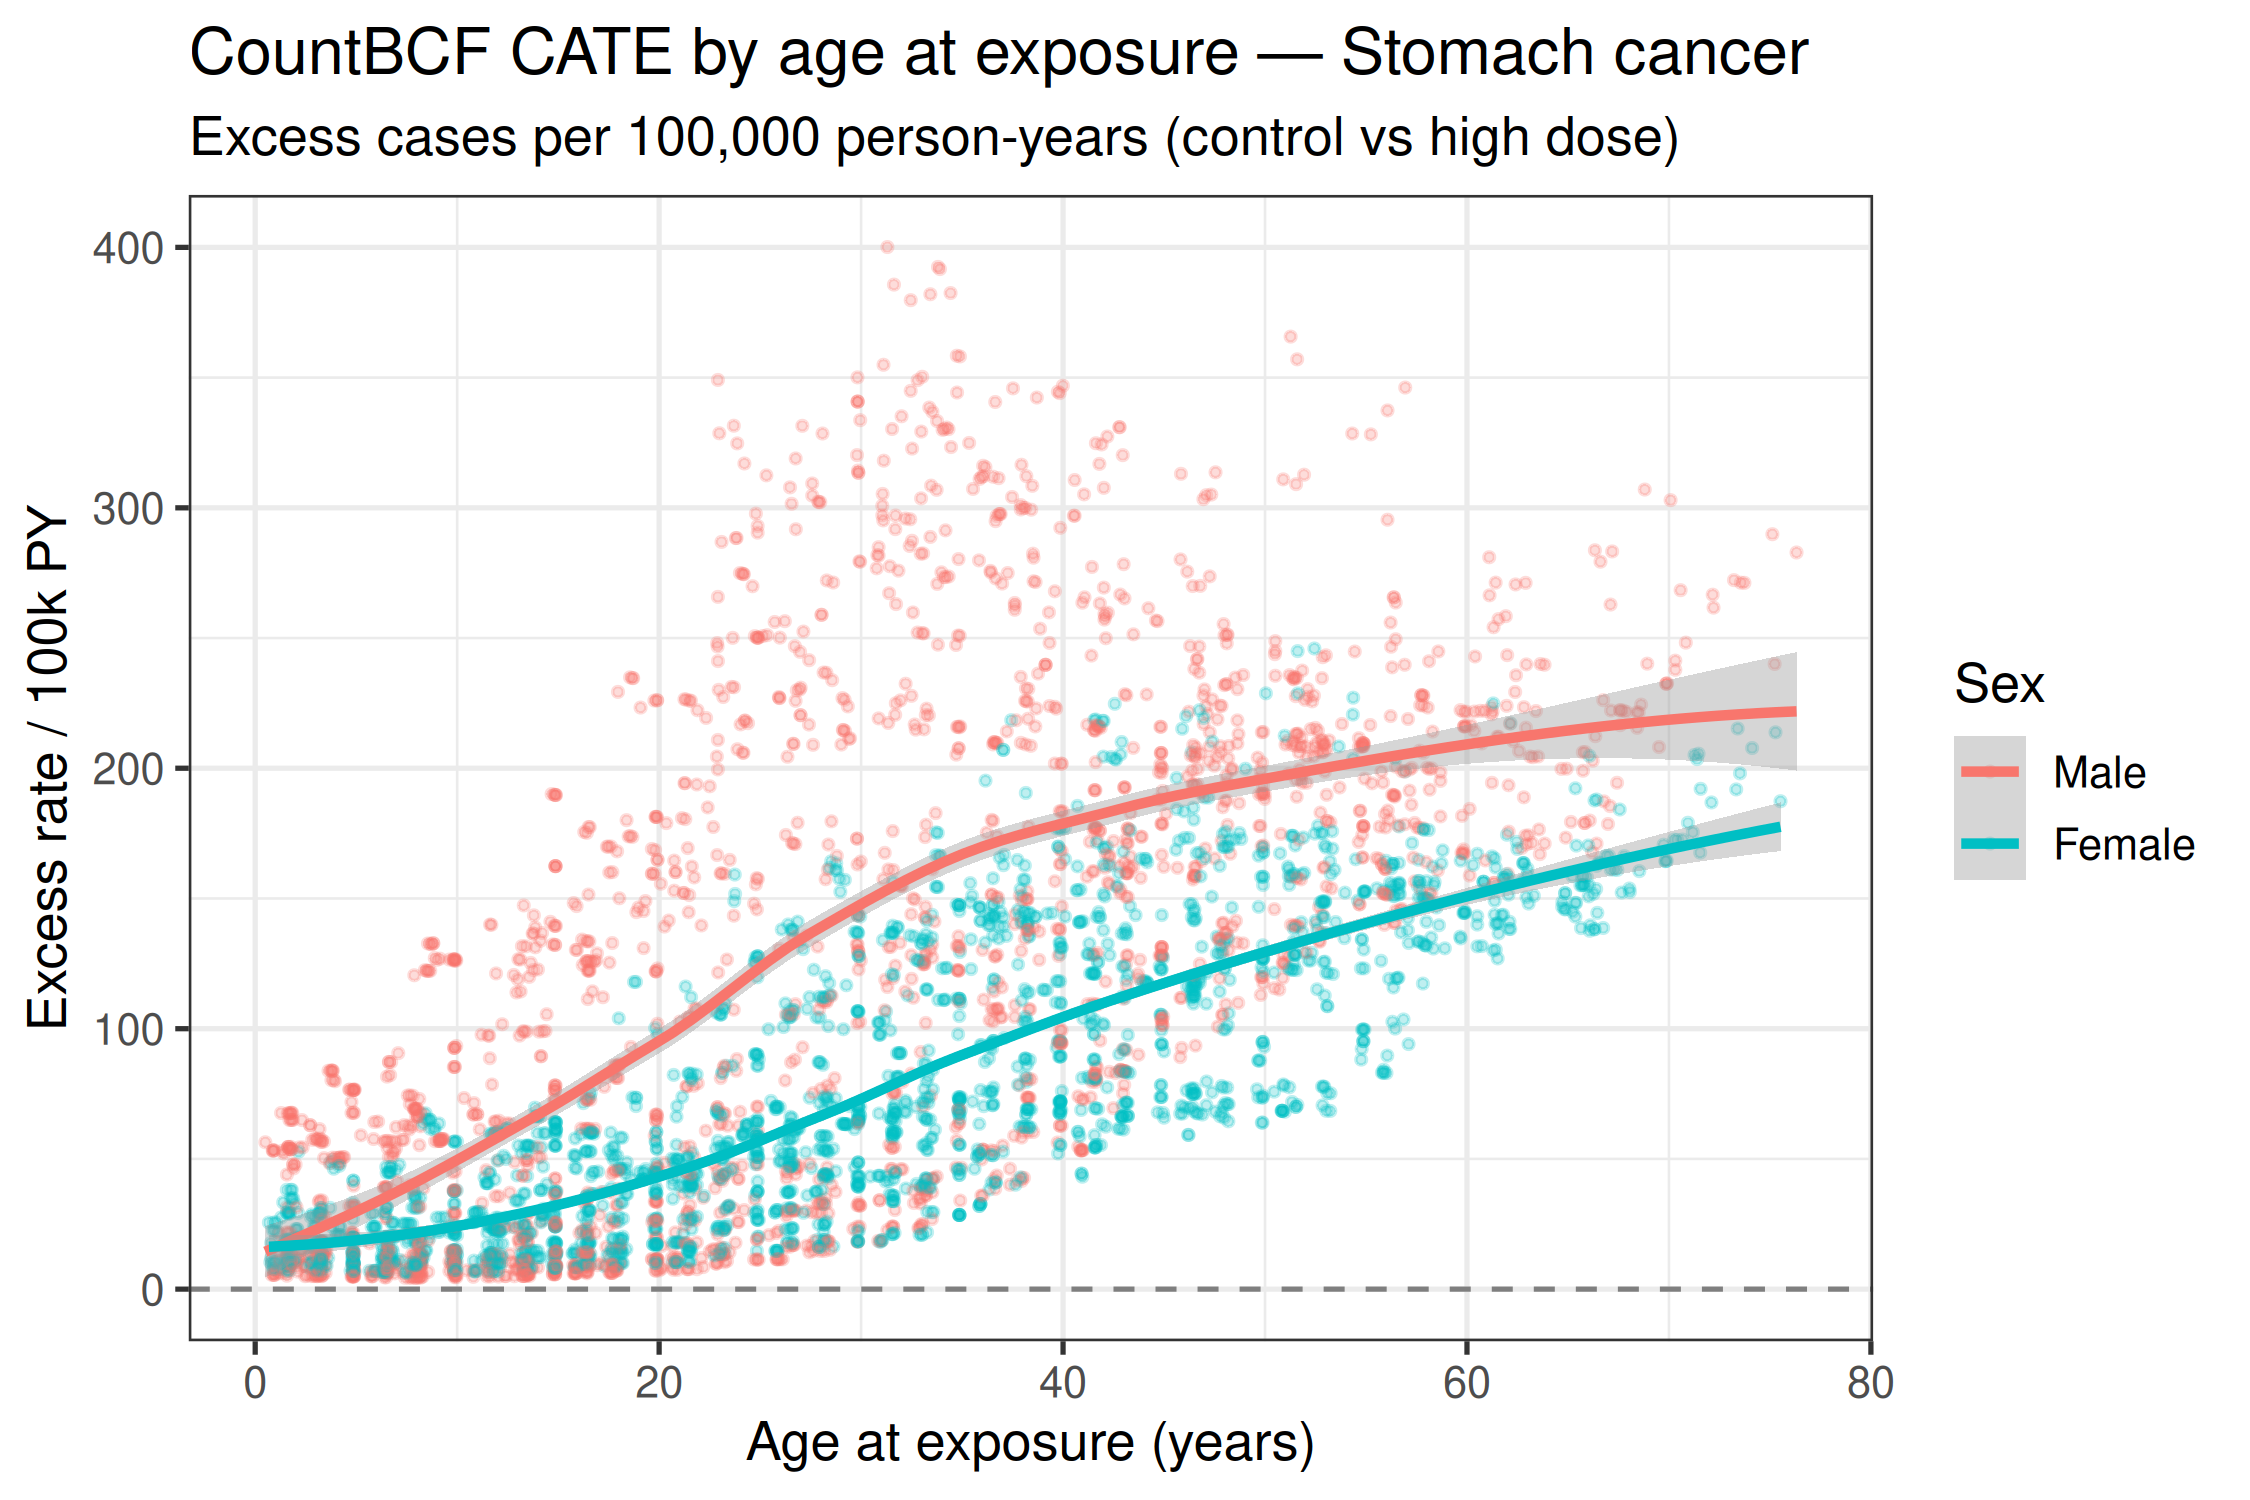
\includegraphics[width=\linewidth]{stomach_cate_by_agex_sex.png}
  \caption{Stomach}\label{fig:ear-agex-stomach}
\end{subfigure}
\caption{\textbf{The EAR--ERR tension on the absolute scale.} Per-cell CATE
(excess cases$/10^5$~PY) against \emph{age at exposure}, by sex. Unlike the
monotone relative-scale decline of Figure~\ref{fig:err-agex}, the
\emph{absolute} excess is non-monotone in age at exposure --- it peaks for
intermediate exposure ages --- because each exposure-age band is observed at a
different attained age (Table~\ref{tab:applied-gradients}). The two scales
therefore rank the exposure-age groups differently.}
\label{fig:ear-agex}
\end{figure}

\begin{figure}[htbp]
\centering
\begin{subfigure}{0.49\textwidth}
  \centering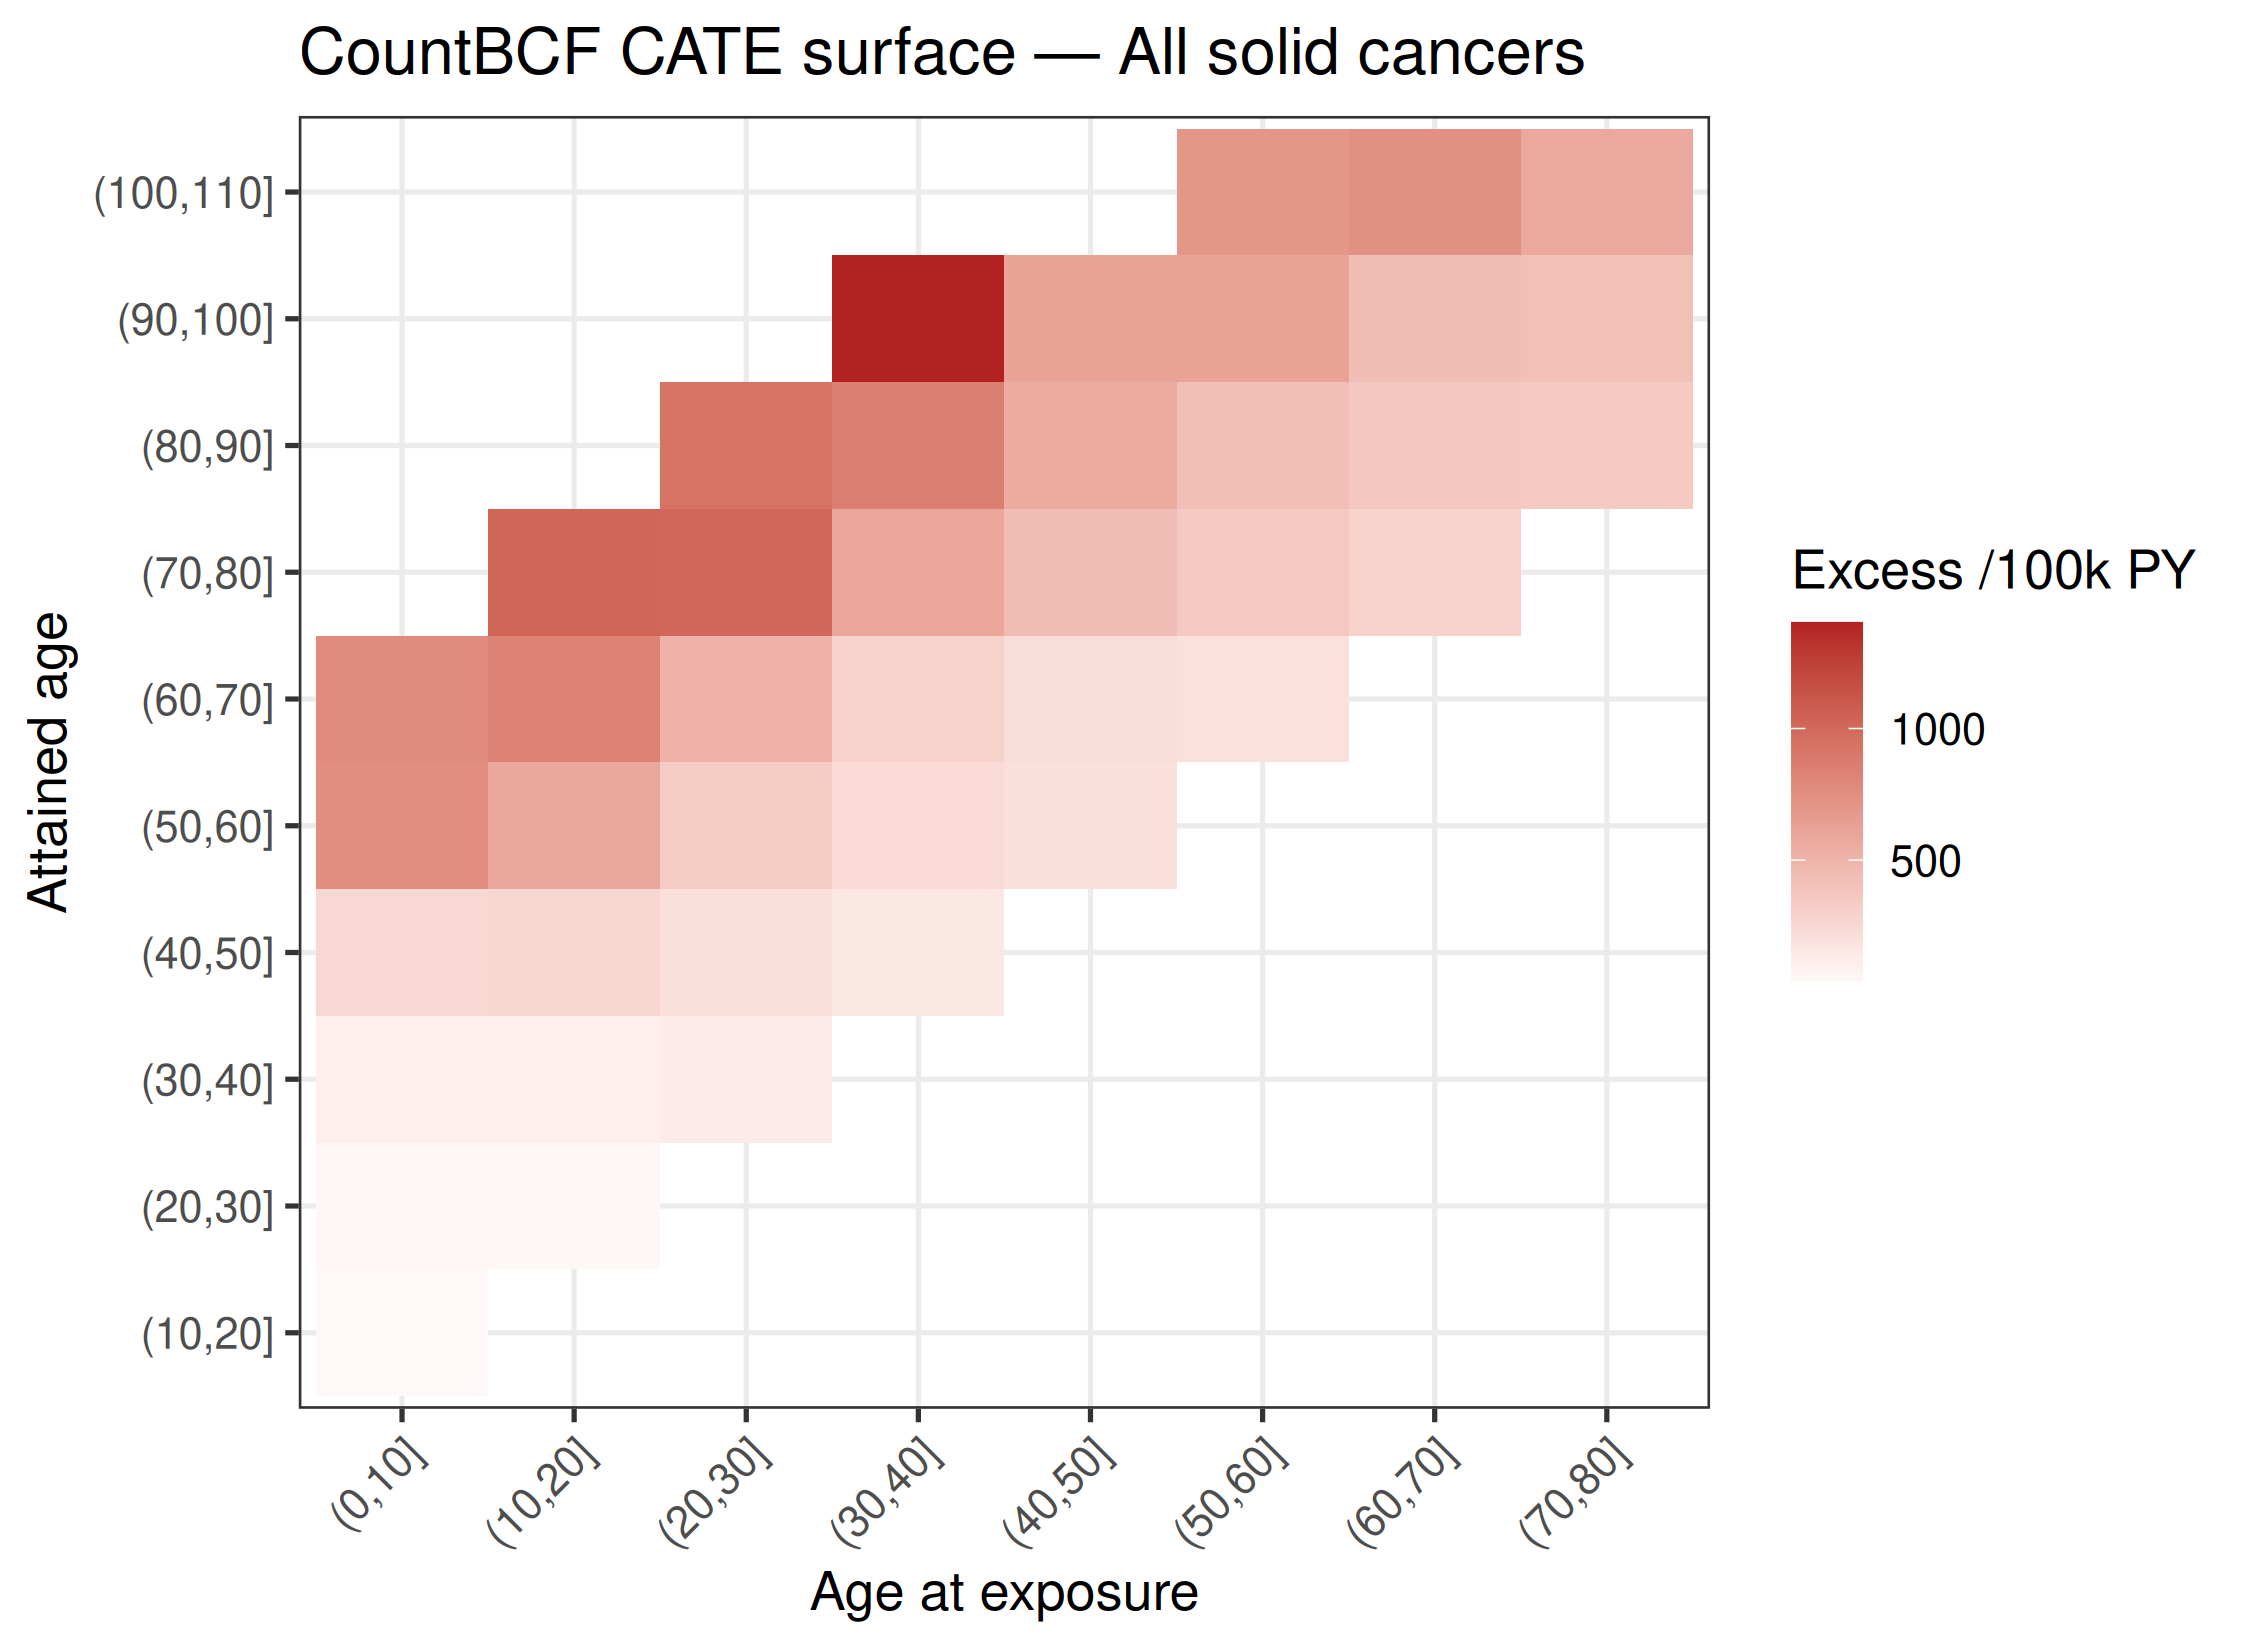
\includegraphics[width=\linewidth]{solid_cate_heatmap.png}
  \caption{All solid cancers}\label{fig:heatmap-solid}
\end{subfigure}
\hfill
\begin{subfigure}{0.49\textwidth}
  \centering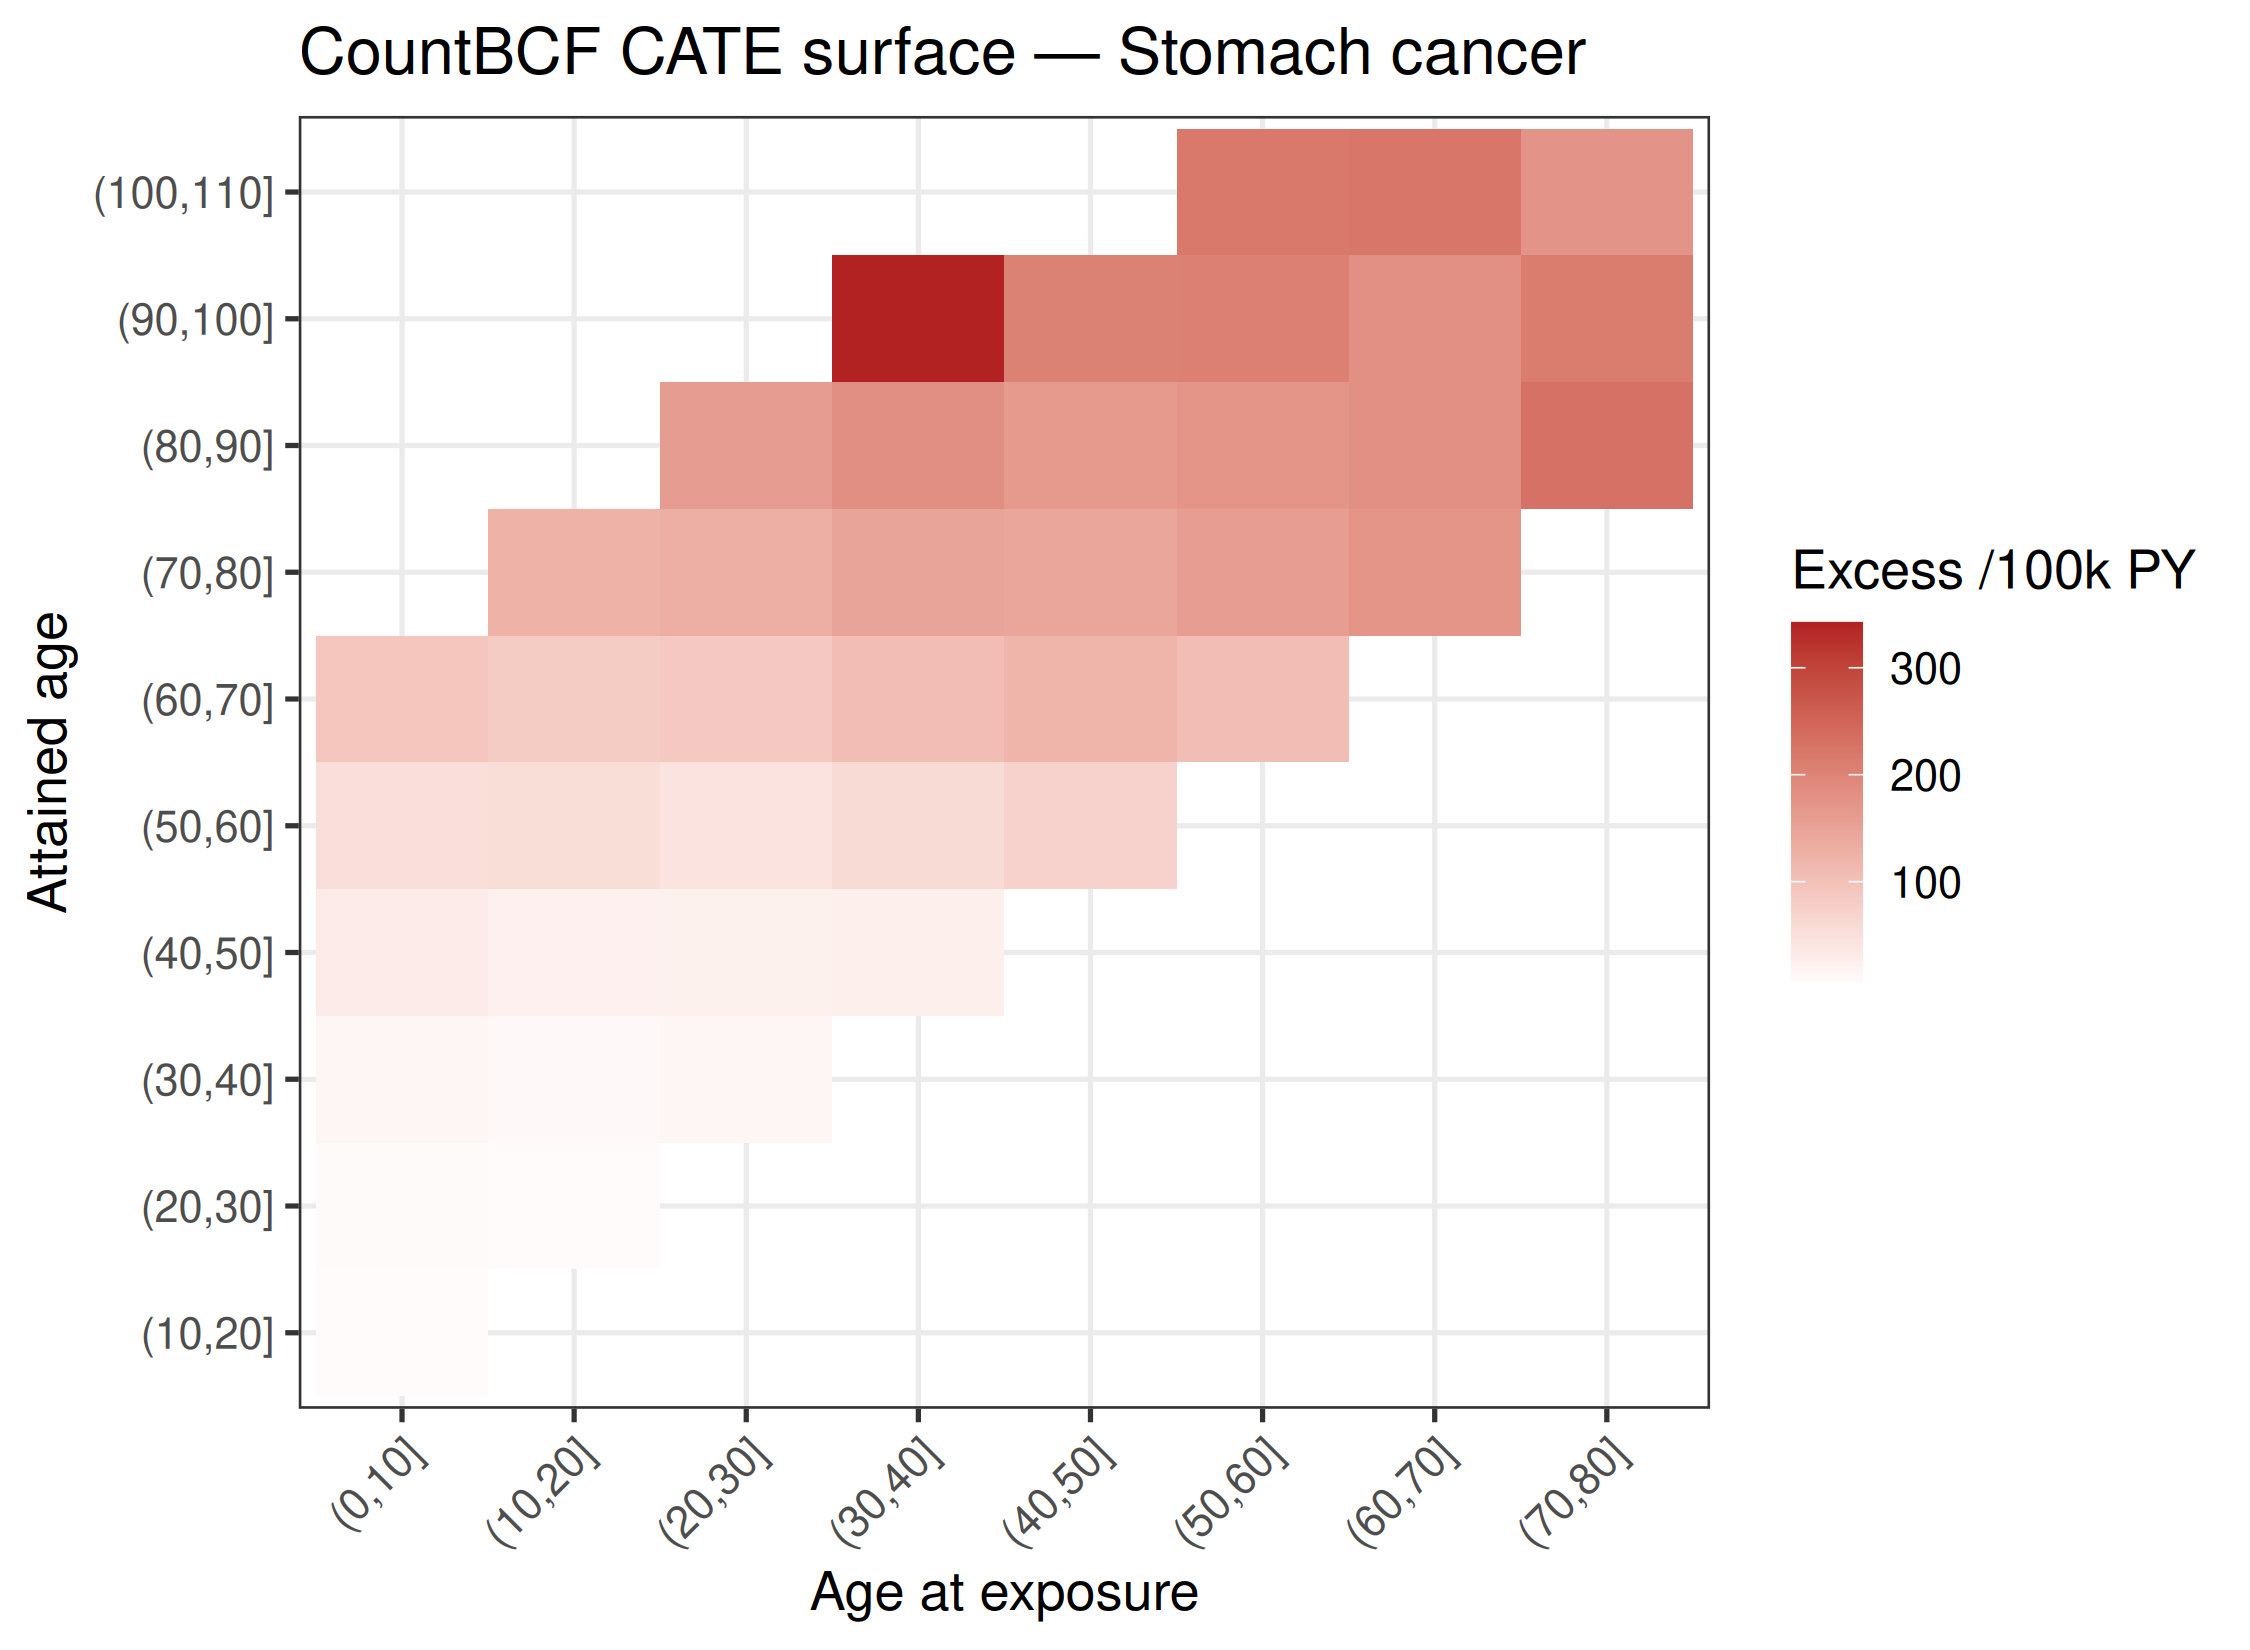
\includegraphics[width=\linewidth]{stomach_cate_heatmap.png}
  \caption{Stomach}\label{fig:heatmap-stomach}
\end{subfigure}
\caption{\textbf{The CATE surface.} Posterior-mean excess cases$/10^5$~PY for
the high-dose contrast over the age-at-exposure $\times$ attained-age plane.
Intensity concentrates toward old attained age and younger-to-middle age at
exposure, the joint maximum of the long-fuse relative effect and the rising
absolute baseline. This two-dimensional surface is the deconfounded object;
the one-dimensional margins of Figures~\ref{fig:err-agex}--\ref{fig:ear-agex}
are projections of it.}
\label{fig:heatmap}
\end{figure}

\subsection{Convergence with the radiation-epidemiology literature}
\label{sec:applied-convergence}

We benchmarked the recovered surface against the canonical LSS comparators
--- the comprehensive solid-cancer incidence reports of
\citet{thompson1994}, \citet{preston2007} and \citet{grant2017}, the mortality
overview of \citet{ozasa2012}, and the site-specific upper-digestive analysis
of \citet{sakata2019} --- supplemented by a structured synthesis of six
independent literature reviews. On the great majority of testable claims
CountBCF converges with the established science, often quantitatively.

The age-at-exposure decline of solid ERR is textbook: \citet{grant2017}
estimate the linear ERR decreases by $\approx 21\%$ per decade increase in
age at exposure (smoking-adjusted), and \citet{preston2007} report
$\approx 17\%$ per decade; CountBCF recovers the same monotone, steep decline
with no interaction term specified. The attained-age rise of EAR, with a
relative effect that fades as the absolute burden grows, is exactly the
persistent-multiplicative-excess picture RERF has reported for decades
\citep{preston2007, ozasa2012}, and the flat-ERR / rising-EAR behaviour over
time since exposure follows from it directly. The stomach endpoint behaves as
the site-specific literature would predict: a much \emph{shallower}
age-at-exposure slope than the all-solid aggregate --- \citet{sakata2019}
find stomach ERR declines with attained age but \emph{not} significantly with
age at exposure --- together with a female-higher stomach ERR ($0.46$ vs.\
$0.35$), matching the significantly higher female stomach ERR reported by
\citet{sakata2019}. The Hiroshima--Nagasaki contrast is a clean null on both
scales, convergent with the modern position that DS02 dosimetry reconciles
the two cities, leaving no residual neutron-RBE city effect on the
rate-ratio scale \citep{preston2007, ds02}; the model was free to split the
cities and chose not to. The dose response is approximately linear across the
moderate-to-high contrast for solid cancer, consistent with the
approximately linear dose response reported for LSS solid cancer
\citep{preston2007, grant2017} --- with the standing caveat that this applied
section deliberately studies a \emph{binary, three-level} design (a
continuous-dose version of CountBCF is deferred to a future paper), so the
linearity reading rests on only three coarse dose bands and cannot adjudicate
the active debate over low-dose \emph{curvature} \citep{cologne2019}. The
moderate-dose stomach null is the expected low-dose attenuation at a weakly
radiogenic, high-baseline site dominated by non-radiogenic promoters
\citep{sakata2019}.

\subsection{Divergences and contested findings}
\label{sec:applied-divergence}

Two findings warrant closer scrutiny. Neither is a failure of the method;
both turn out to be informative about the estimand and the state of the
literature.

\paragraph{The solid-cancer sex ERR (the substantive divergence).} The
canonical LSS result is that female ERR exceeds male ERR for all-solid
cancer: \citet{preston2007} report a female-to-male ratio of $\approx 1.6$
(rates increasing $35\%$/Gy for men vs.\ $58\%$/Gy for women at age $70$ after
exposure at age $30$), and \citet{grant2017} a still larger ratio under their
sex-specific preferred models. CountBCF instead finds male ERR marginally
\emph{above} female for the colon-dosed solid aggregate ($0.83$ vs.\ $0.76$;
female-to-male $\approx 0.91$) --- a genuine divergence in direction. A
sequence of sensitivity fits on the same data
(Table~\ref{tab:applied-sexsens}) locates its cause precisely, and the cause
is \emph{not} that our aggregate omits the female-driving sites.

First, a construction check confirms that breast and thyroid --- the highly
radiogenic, female-skewed sites that carry much of the female all-solid
excess \citep{brenner2018, furukawa2013, ron1995} --- are \emph{included} in
the RERF all-solid count, not removed: across all $8{,}042$ table cells the
all-solid count is never smaller than the sum of its named constituent sites
including breast and thyroid, which together account for $97.6\%$ of the
total, with non-melanoma skin the one canonical exclusion
(Figure~\ref{fig:sex-construction}). They are present,
but \emph{dosed by the colon surrogate}. This is decisive for the
interpretation, because Preston's all-solid endpoint is \emph{also}
colon-dose-anchored and \emph{also} includes breast and thyroid, yet still
recovers the female-higher ERR --- so colon anchoring \emph{alone} cannot be
the explanation.

\begin{figure}[htbp]
\centering
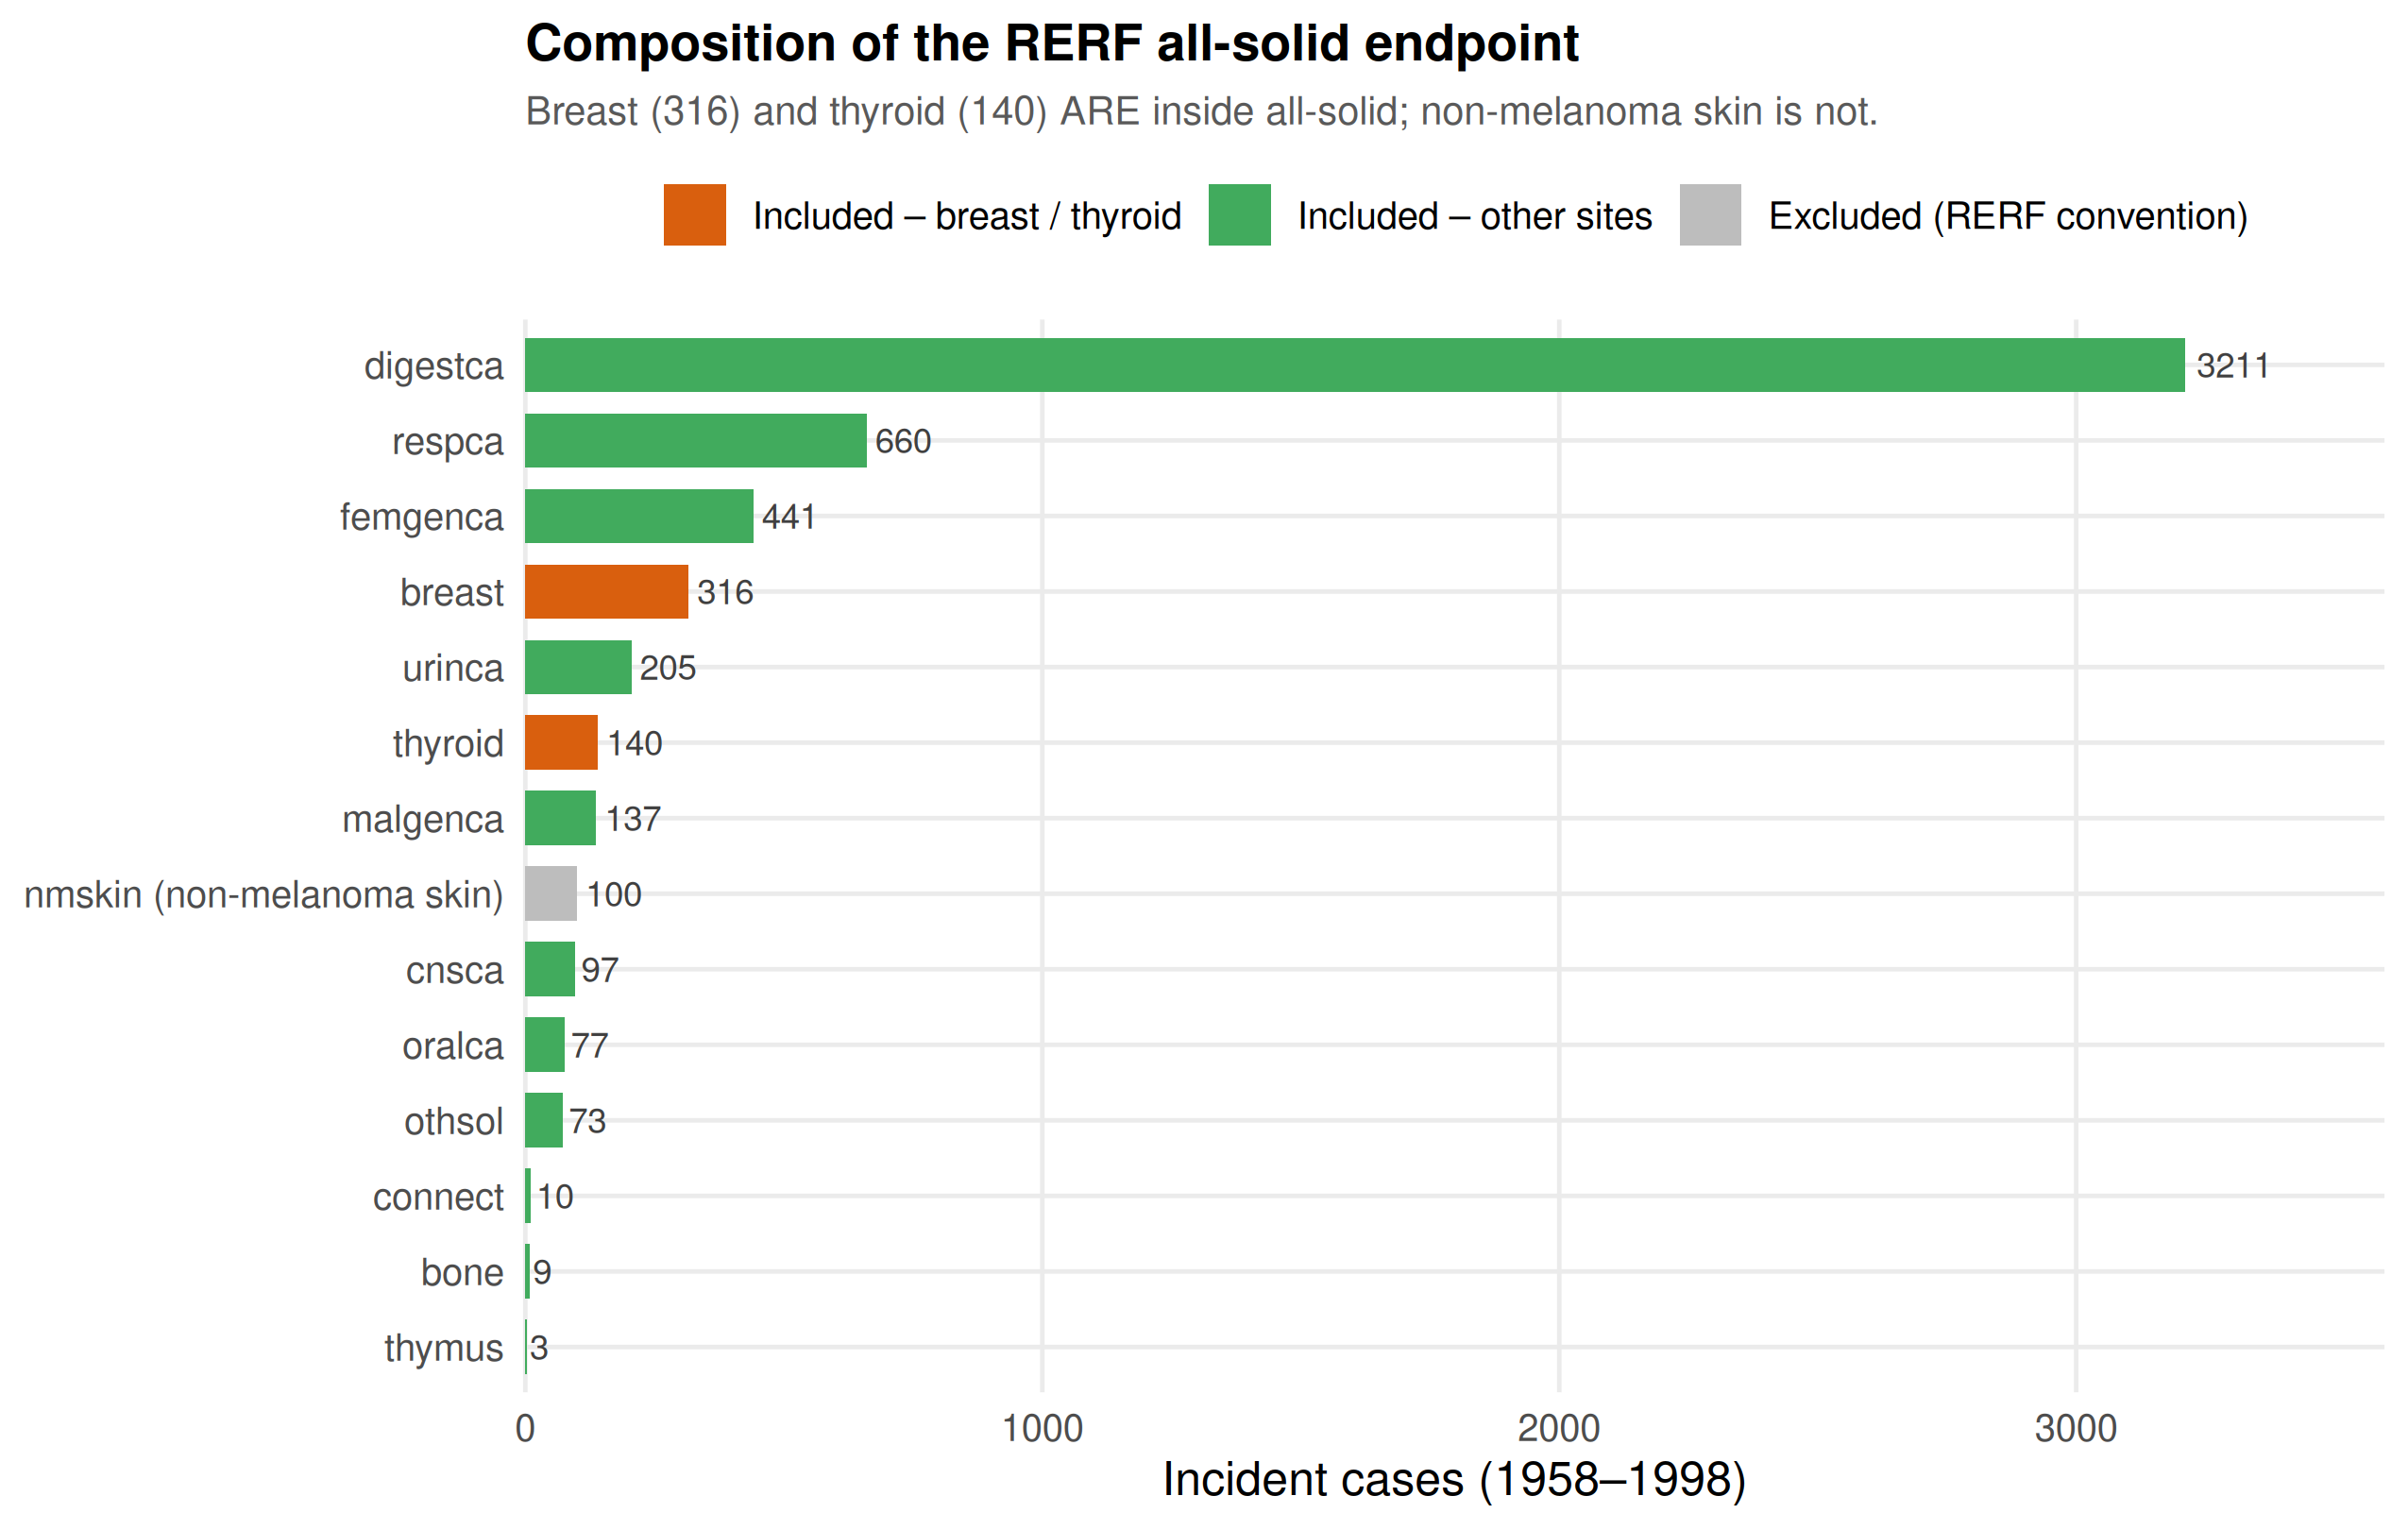
\includegraphics[width=0.82\textwidth]{B1_allsolid_construction.png}
\caption{\textbf{The RERF all-solid endpoint includes the female-driving sites.}
Incident-case composition of the all-solid count over the 1958--1998 follow-up.
Breast ($316$ cases) and thyroid ($140$) --- the highly radiogenic,
female-skewed sites --- are constituent members of the aggregate (orange), not
exclusions; non-melanoma skin ($100$ cases) is the one canonical exclusion
(grey). The named sites shown account for $97.6\%$ of the all-solid total. The
female-driving sites are therefore \emph{present} in our endpoint, but carried
at the colon-dose surrogate rather than their own organ dose.}
\label{fig:sex-construction}
\end{figure}

What colon-dosing does is \emph{dilute} the sites whose radiation signal is
sex-skewed. Fitting breast with its own organ dose recovers a strong female
ERR (NB GLM $1.63$ $[0.83, 2.78]$; CountBCF $\approx 1.1$;
Table~\ref{tab:applied-sexsens}; Figure~\ref{fig:sex-owndose}), and thyroid
likewise shows a large radiation
effect with its own dose --- the method plainly ``sees'' the sex-relevant
signal when the dose is right. Inside the
colon-dosed aggregate, however, that signal is flattened toward the common
$\approx 0.8$ colon ERR. Consistent with this, removing breast and thyroid
from the colon-dosed aggregate barely moves the sex ratio (female-to-male
$0.91 \to 0.92$): in our endpoint those sites neither carry nor, when removed,
change the female excess, precisely because they are dose-diluted --- the
mirror image of Preston's properly-dosed analysis, in which restricting to
non-gender-specific cancers \emph{removes} the female excess
\citep{preston2007, walsh2016}.

\begin{figure}[htbp]
\centering
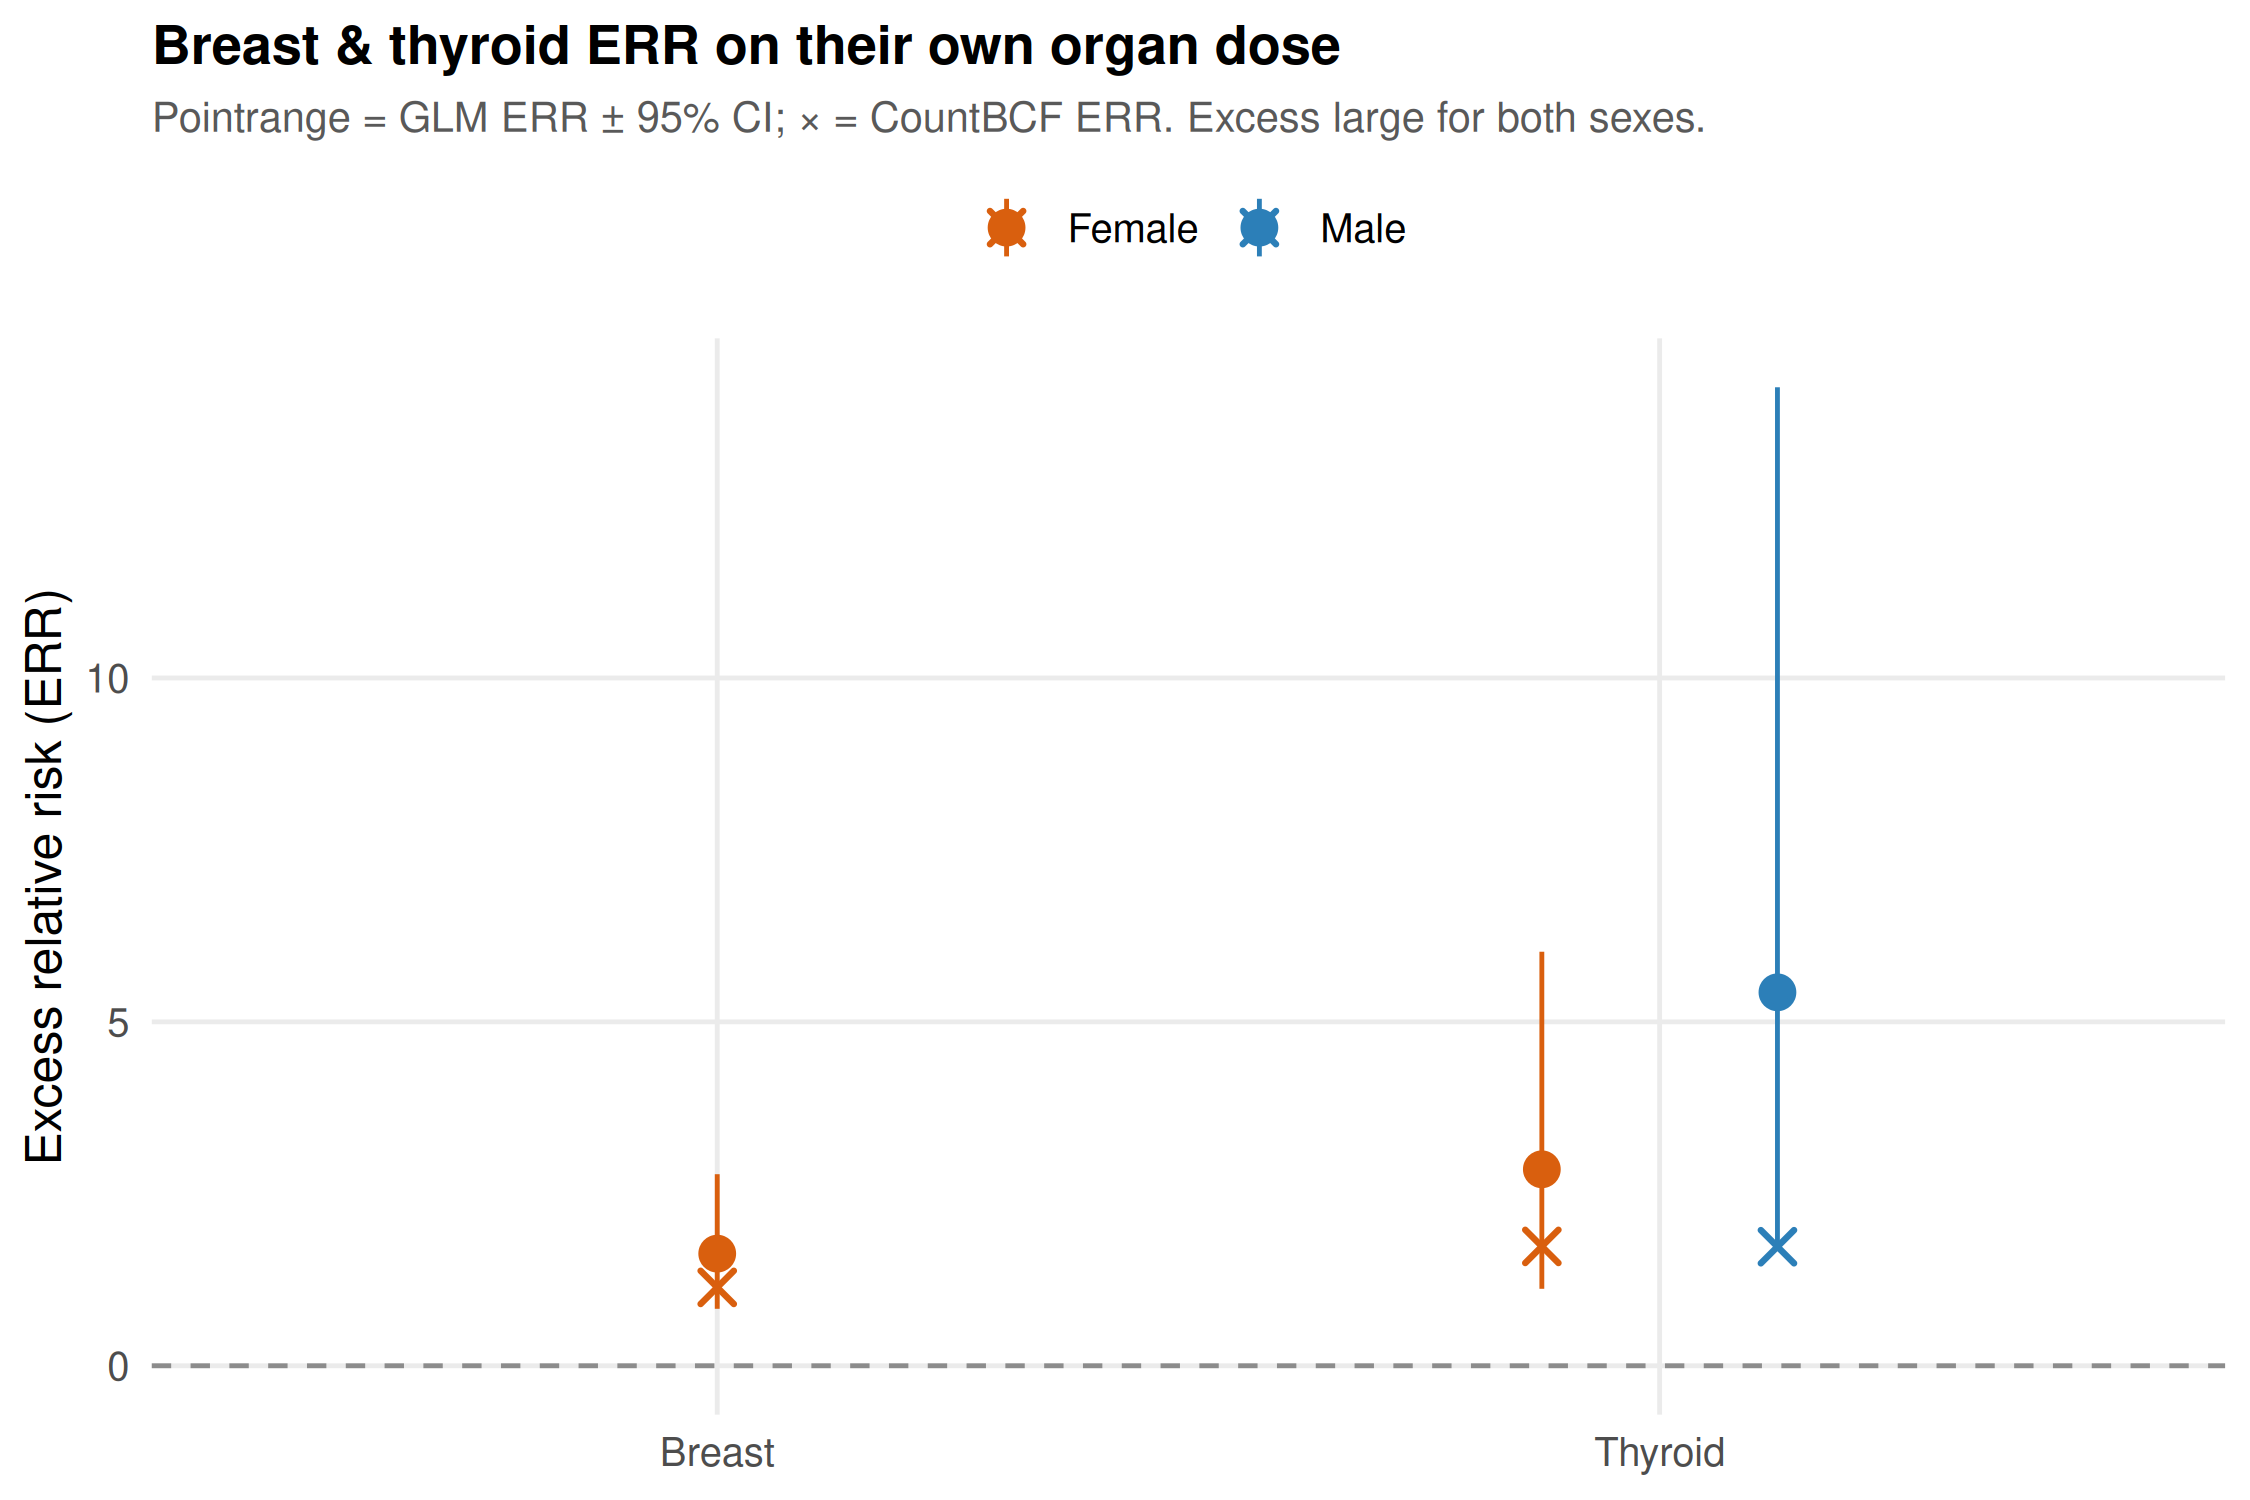
\includegraphics[width=0.62\textwidth]{B2_breast_thyroid_err.png}
\caption{\textbf{On their own organ dose, the female-driving sites show their
signal.} Excess relative risk for breast and thyroid fitted with their
\emph{own} organ dose (high-dose contrast), by sex: point-ranges are the NB-GLM
ERR with $95\%$ confidence intervals, crosses ($\times$) the corresponding
CountBCF posterior-mean ERR. Breast carries a strong female excess (GLM ERR
$1.63$) and thyroid a large --- if imprecisely estimated --- effect in both
sexes. This is the sex-relevant signal that the colon-dosed aggregate flattens
toward its common $\approx 0.8$ ERR, and it is recovered automatically once the
dose is the correct one.}
\label{fig:sex-owndose}
\end{figure}

The residual male tilt is then a \emph{design} artifact, not a property of the
sites or of colon anchoring. Two design choices reverse it. Relaxing the
$2$~Gy dose cap to $4$~Gy lifts the female ERR above the male and flips the
ratio to female-higher (female-to-male $\approx 1.30$); moving the high-dose
band to $\geq 1$~Gy does the same ($\approx 1.25$;
Figure~\ref{fig:sex-design}). The canonical
female-higher direction is therefore recovered once the highest doses --- which
our $2$~Gy truncation and coarse three-level binning discard or blunt --- are
retained, and the residual tilt is further consistent with the younger mean
attained age of our capped high-dose subset, at which the steep late-life
attenuation of the male ERR has not yet occurred. A complementary
contribution is that pooling etiologically heterogeneous sites under one
background-rate model can distort marginal sex patterns \citep{cologne2019}.
In short, the divergence is explained by dose-surrogate dilution of the
female-driving sites together with our $2$~Gy / three-level design, reverses
under a wider dose range, and is not a contradiction of the radiobiology.
Authoritative confirmation that our all-solid case definition matches the
Preston/Grant endpoint remains a codebook item for the domain co-authors.

\begin{table}[htbp]
\centering
\caption{Sex-ERR sensitivity for the high-dose contrast
(person-year-weighted ERR by sex). The primary colon-dosed all-solid result
is mildly male-leaning (female-to-male $\approx 0.91$); \emph{excluding}
breast and thyroid leaves it essentially unchanged, but relaxing the $2$~Gy
cap or raising the high-dose threshold \emph{reverses} it to the canonical
female-higher direction, and breast fitted with its own organ dose recovers a
strong female ERR. Per-sex ERR \emph{levels} carry Monte-Carlo variation
across independent fits (the primary baseline below reproduces the
female-to-male $\approx 0.91$ of the main analysis); the female-to-male
\emph{ratio} is the stable, inferentially relevant quantity.}
\label{tab:applied-sexsens}
\small
\begin{tabular}{lccc}
\toprule
Specification (high-dose contrast) & Male ERR & Female ERR & Female:Male \\
\midrule
All-solid, colon dose, $\leq 2$~Gy, bands $.1/.5$ (primary) & 0.92 & 0.83 & 0.91 \\
\quad excluding breast \& thyroid (colon dose)              & 0.57 & 0.53 & 0.92 \\
\quad dose cap relaxed to $4$~Gy                             & 0.77 & 1.00 & \textbf{1.30} \\
\quad high-dose band $\geq 1$~Gy                             & 0.94 & 1.18 & \textbf{1.25} \\
\quad finer control cut ($<0.05$~Gy)                         & 0.90 & 0.83 & 0.93 \\
\midrule
Breast alone, own organ dose (female, NB GLM) & \multicolumn{2}{c}{ERR $1.63$ $[0.83,\,2.78]$} & --- \\
\bottomrule
\end{tabular}
\end{table}

\begin{figure}[htbp]
\centering
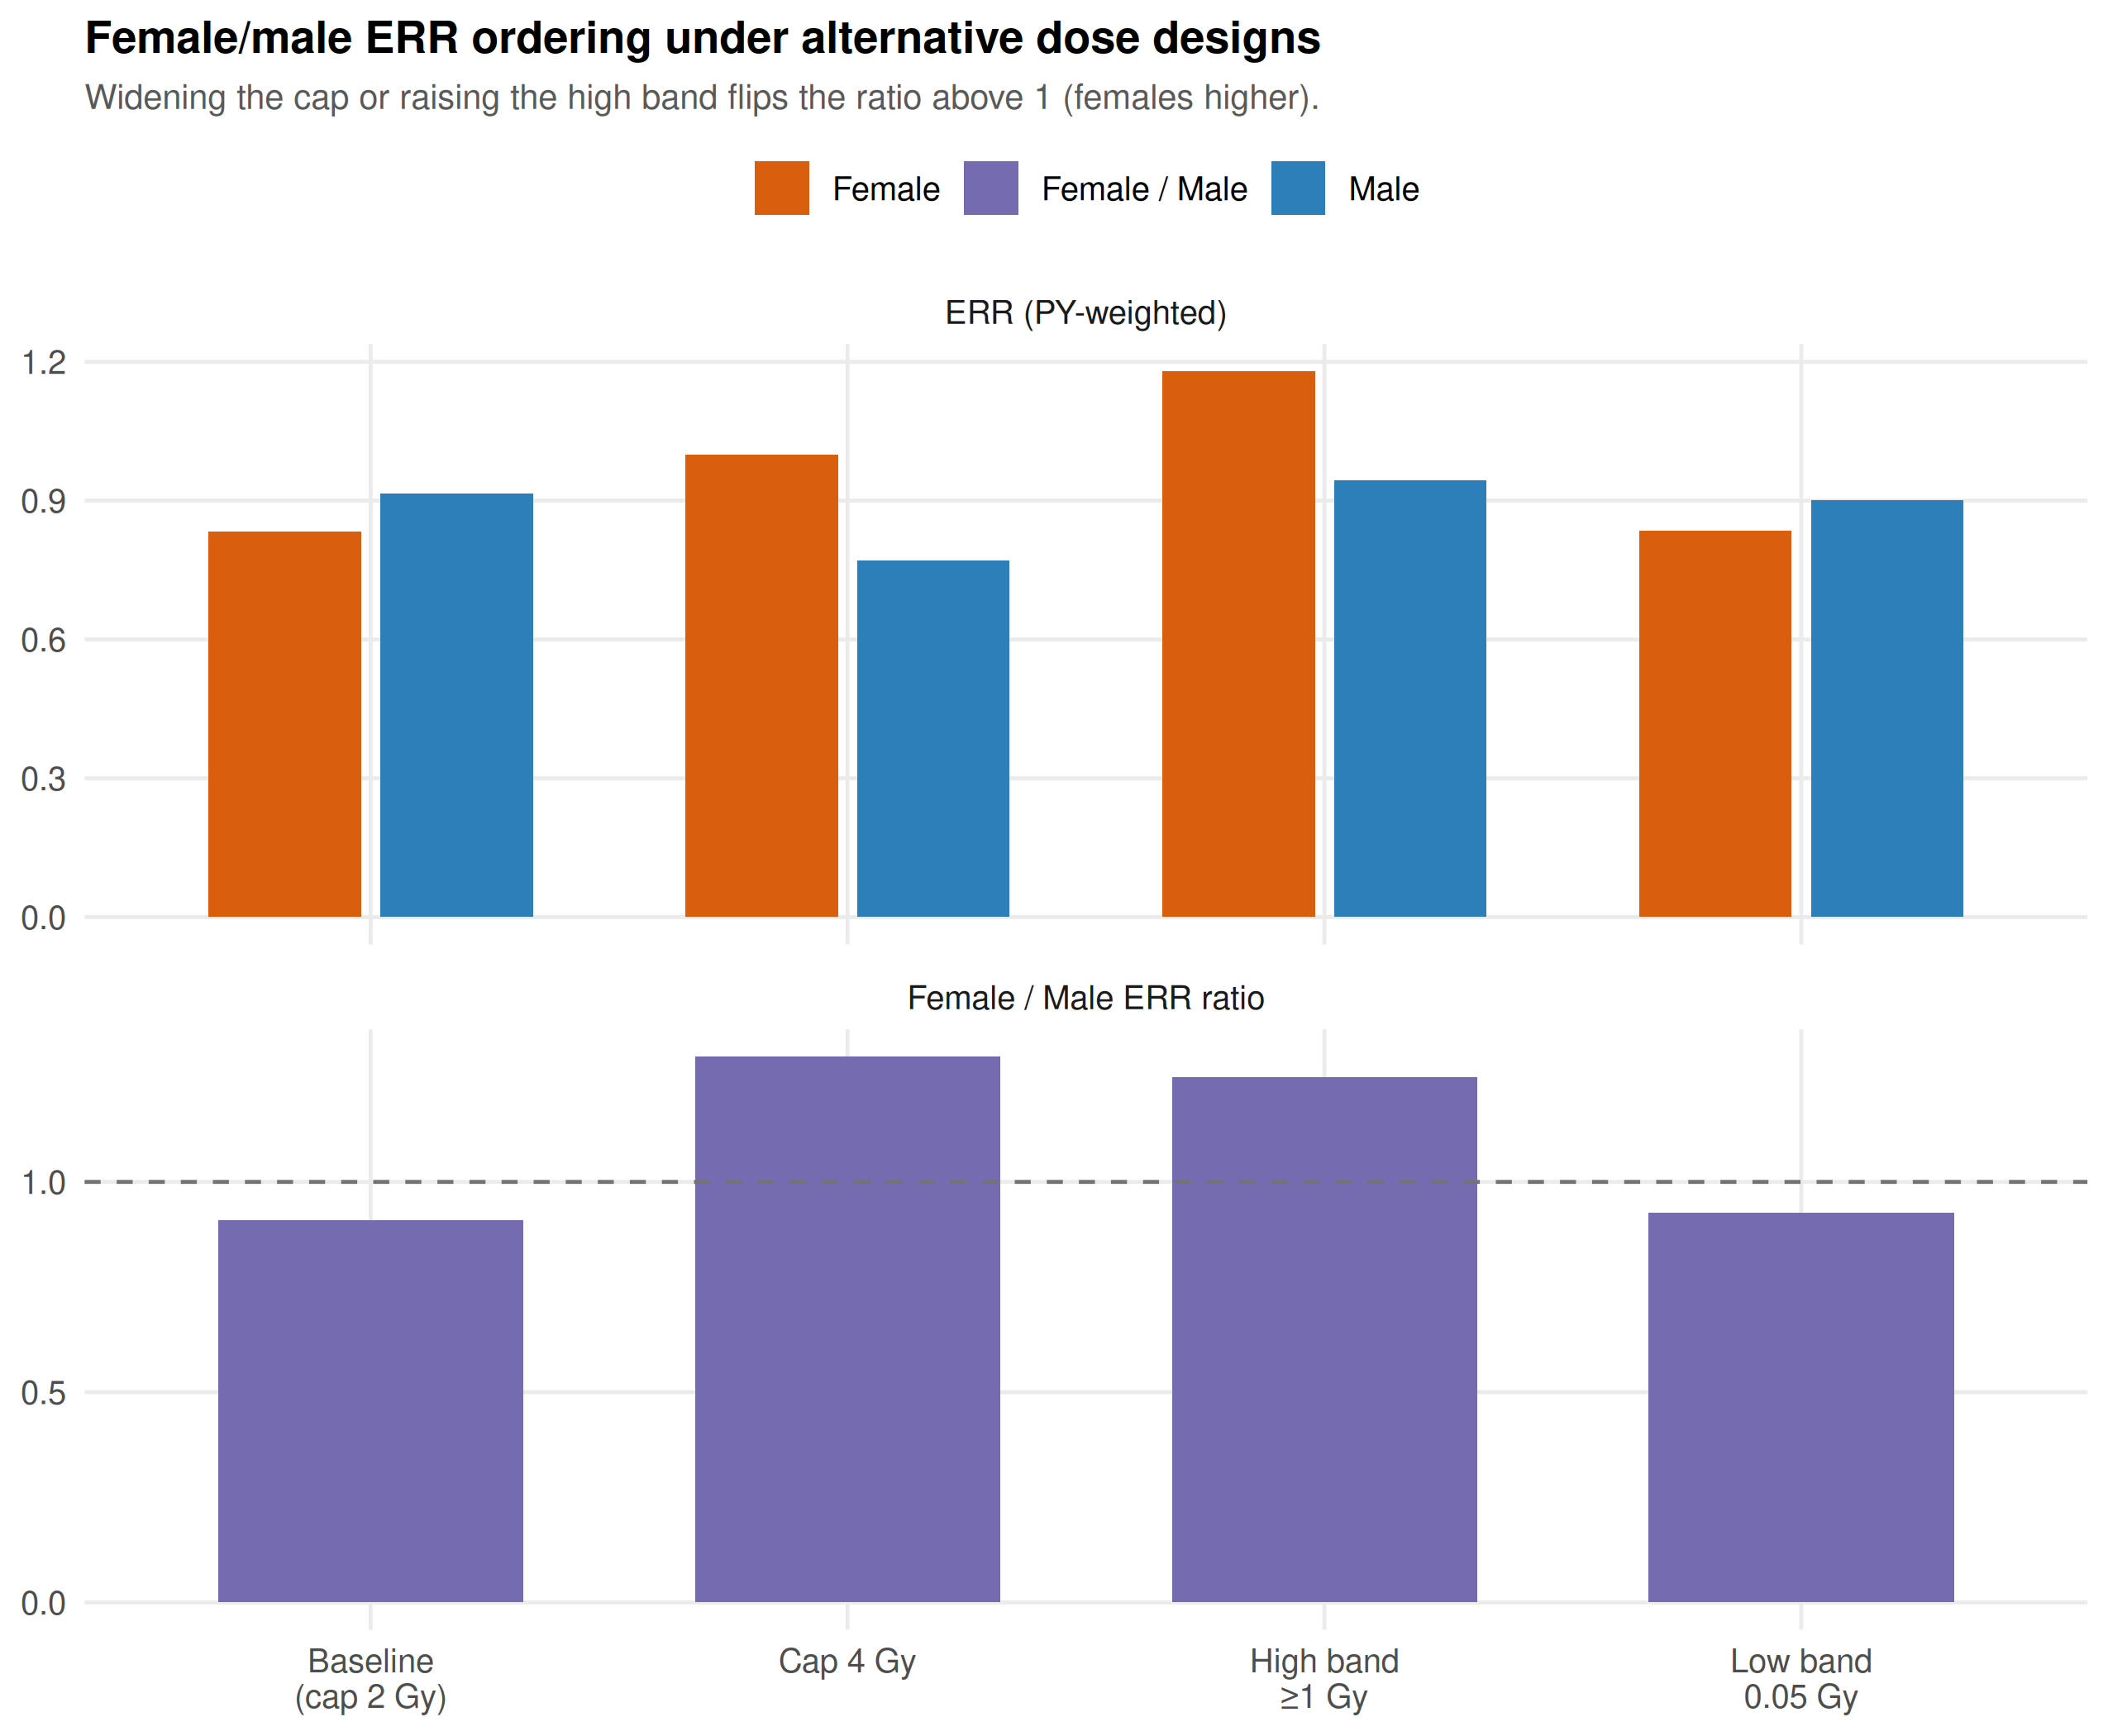
\includegraphics[width=0.74\textwidth]{B4_design_sensitivity.png}
\caption{\textbf{The residual male tilt is a design artefact.} \emph{Top:} per-sex
person-year-weighted ERR for the high-dose contrast under four dose-design
choices. \emph{Bottom:} the female-to-male ERR ratio for each (dashed line at
parity). The primary $2$~Gy-capped, three-level design leaves the ratio just
below $1$ (male-leaning); widening the cap to $4$~Gy or moving the high-dose band
to $\geq 1$~Gy lifts the female ERR above the male and flips the ratio to the
canonical female-higher direction ($\approx 1.30$ and $\approx 1.25$), whereas a
finer control cut does not. The plotted values are those of
Table~\ref{tab:applied-sexsens}.}
\label{fig:sex-design}
\end{figure}

\paragraph{The age-at-exposure plateau and faint upturn (a contested
shape).} CountBCF finds the solid ERR decline arresting around
age-at-exposure $40$--$50$ and flattening to a plateau of $\approx 0.25$,
with a faint upturn at the oldest exposure ages, rather than the strictly
log-linear decline-toward-zero of the simplest parametric modifier. This
diverges only from the textbook default, not from the literature as a whole.
\citet{shuryak2010} argue directly that for exposures in adulthood the
relative risks ``generally do not decrease monotonically with increasing age
of adult exposure,'' inconsistent with standard log-linear models; the BEIR
VII committee institutionalised a model in which the modifier is
\emph{constant} above age $30$ rather than continuing to decline
\citep{beirvii2006}; and \citet{grant2017} themselves fit competing
spline and plateau-after-$30$ parameterizations whose fit is not decisively
worse than the log-linear form. CountBCF's answer --- plateau, with a hint of
upturn --- thus aligns with a recognised, named body of LSS modelling rather
than contradicting it. Three considerations temper the claim, and together
they place the upturn somewhere between data artifact, biology and a mix of
the two. First, the upturn may be an \emph{aggregation artifact}:
\citet{little2009} shows that the apparent non-monotonic variation of relative
risk with age at exposure in the all-solid aggregate weakens to only marginal
significance once cancer sites are stratified ($P=0.060$ for incidence), so
pooling etiologically heterogeneous sites under one background-rate model can
manufacture exactly this edge feature --- the age-at-exposure analogue of the
background-heterogeneity concern of \citet{cologne2019} already raised for the
sex result. We see the same signature in our own data: re-fitting individual
sites with their own organ doses, the steep age-at-exposure decline of the
aggregate \emph{does not} reappear --- colon and lung ERR are essentially flat
(indeed faintly rising) across age at exposure
(Figure~\ref{fig:site-agex}) --- so the aggregate's strong
gradient and its old-age curvature are substantially a property of the
\emph{mixture}, not of any constituent site. Second, the oldest-exposed
stratum is the sparsest (the $60+$ band
carries only $\sim$7\,800 PY against $\sim$183\,000 for the $10$--$20$ band),
so the upturn is weakly identified and prior-influenced: CountBCF shrinks such
sparse cells \emph{toward the positive global mean effect}, which can by
itself lift the oldest, data-poorest band and create an apparent upturn where
the data are nearly silent. The posterior intervals accordingly balloon in the
oldest-exposed ($40+$) band, and for solid-cancer females the lower bound
touches zero (Figure~\ref{fig:subgroups}). Third, one-dimensional
age-at-exposure margins are entangled with attained age, so part of the
apparent flattening may be a projection of the joint surface rather than a
feature of it \citep{grant2017}. We therefore present the plateau as
convergent with BEIR VII / \citet{shuryak2010} and the faint upturn as a
hypothesis-generating edge effect --- data artifact, biology, or a mix --- not
a firm result.

\begin{figure}[htbp]
\centering
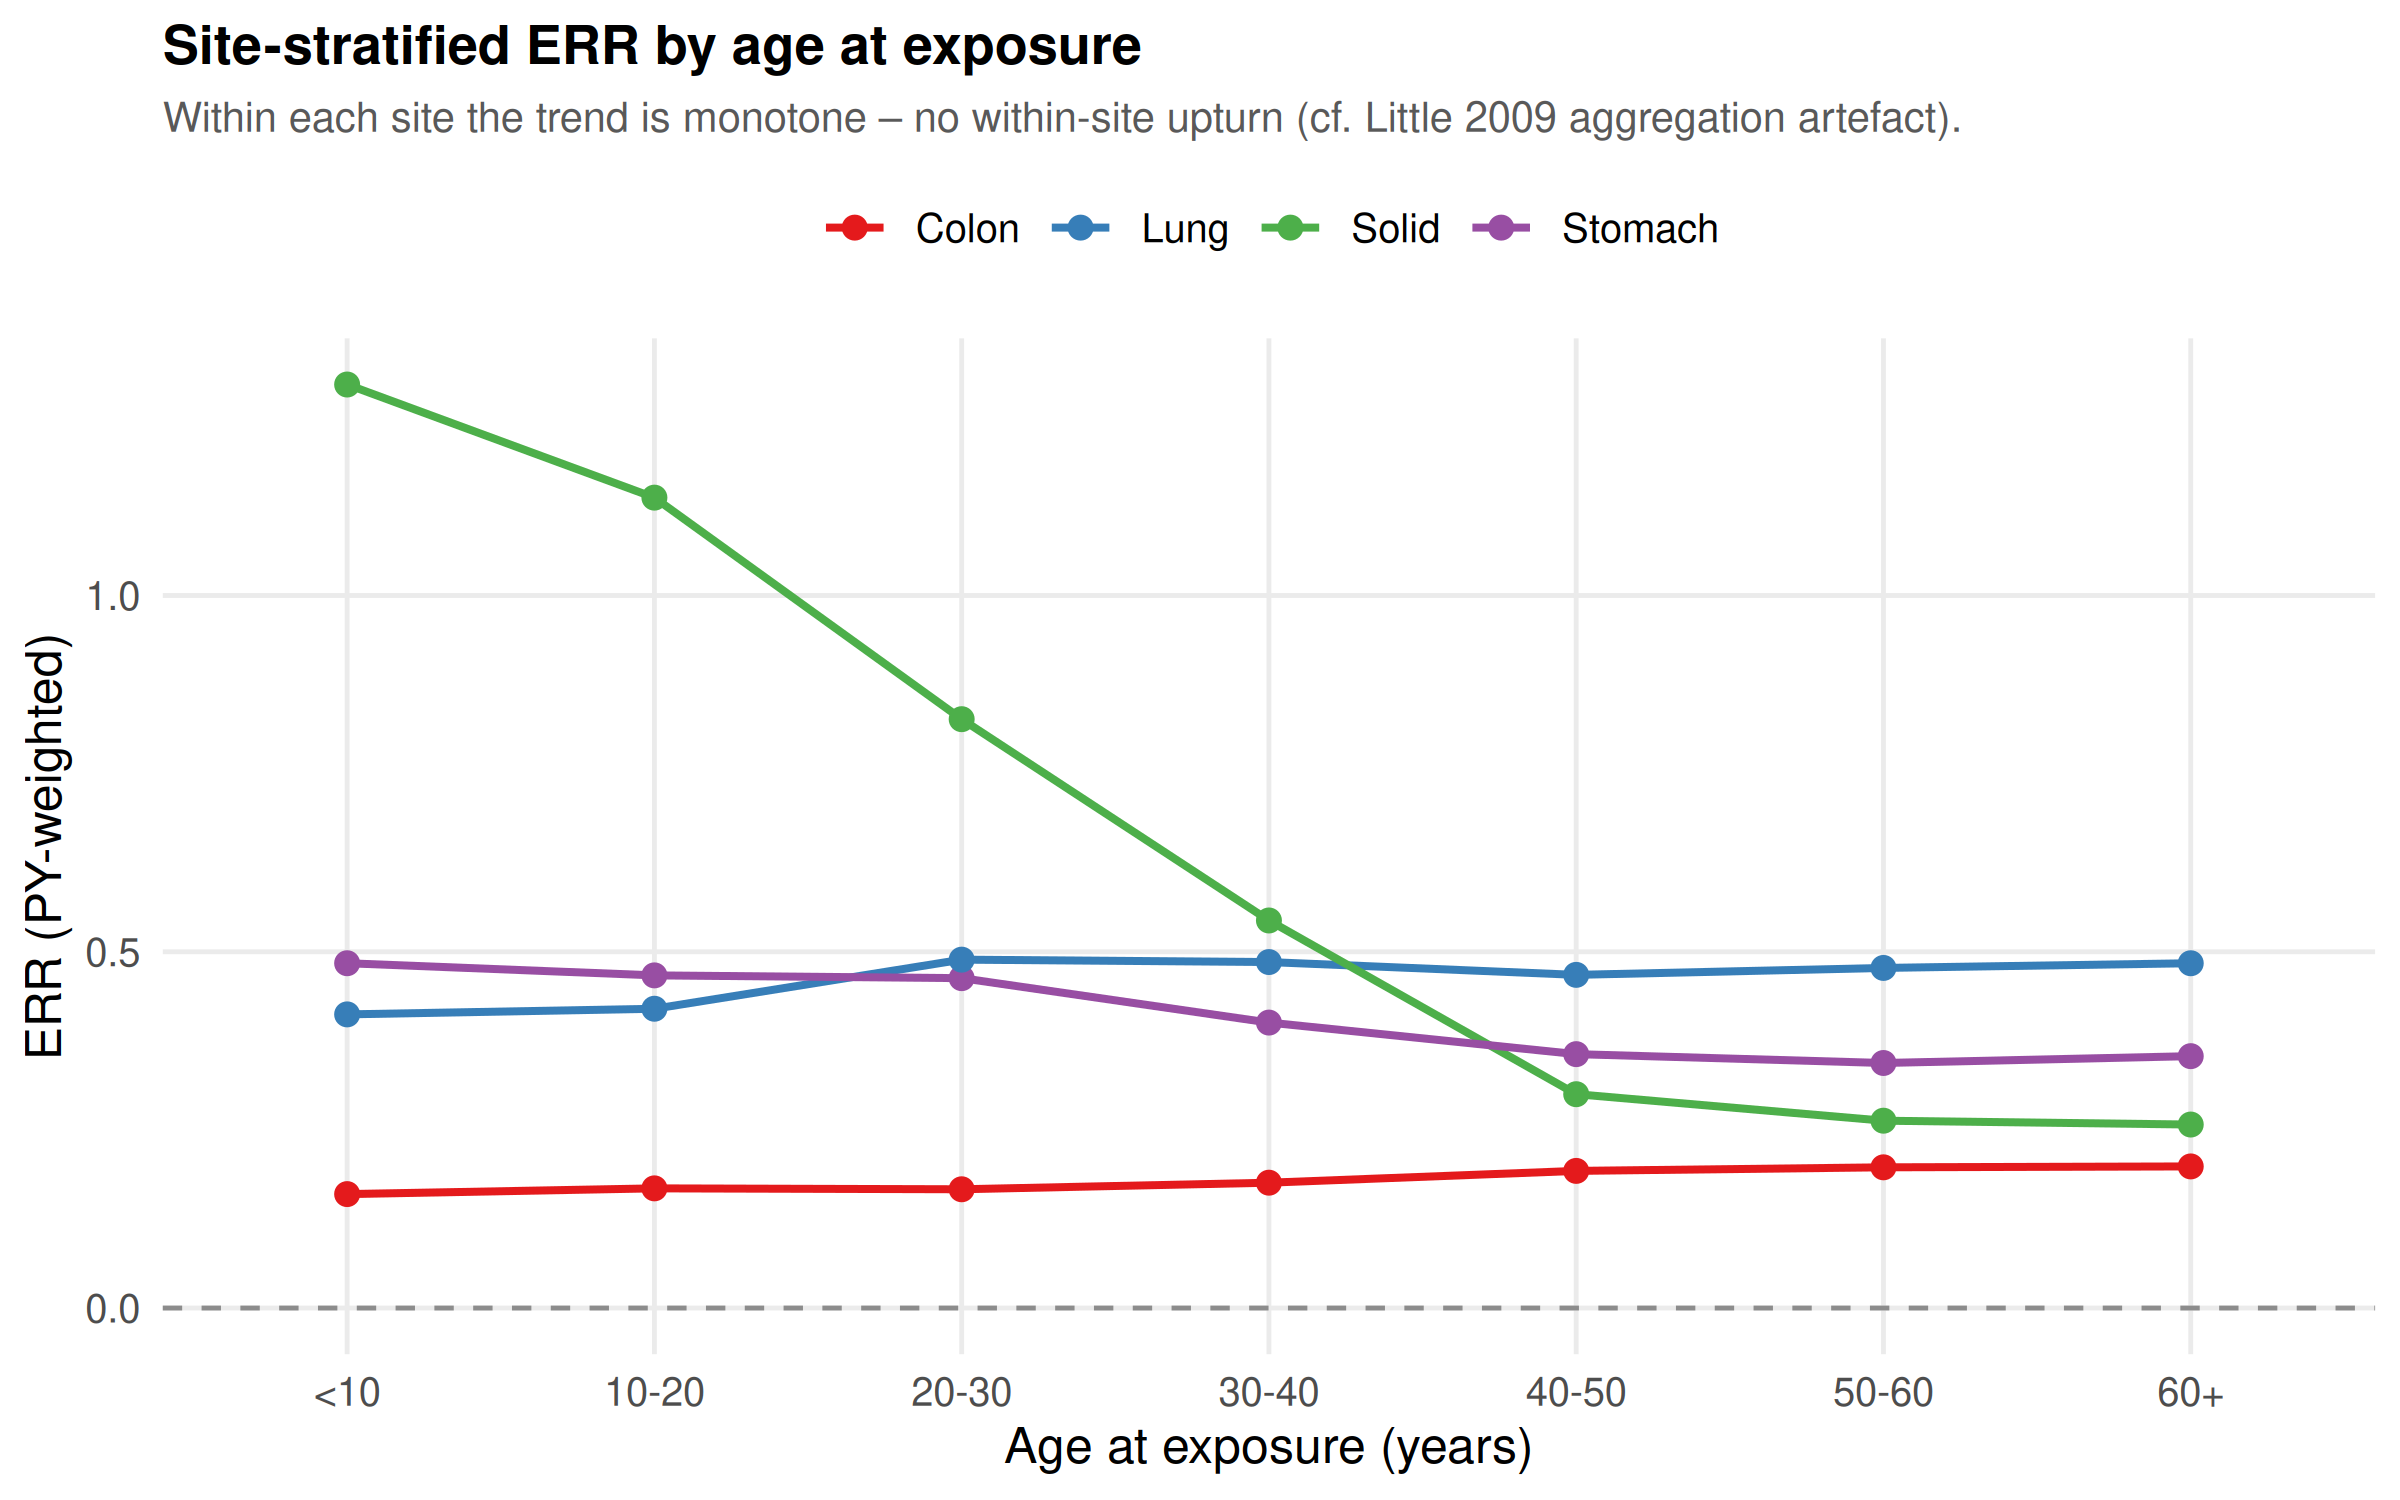
\includegraphics[width=0.82\textwidth]{B7_site_stratified_agex.png}
\caption{\textbf{The age-at-exposure gradient is largely a mixture effect.}
Person-year-weighted ERR for the high-dose contrast against age at exposure,
each cancer site fitted with its \emph{own} organ dose. The steep decline of the
colon-dosed all-solid aggregate (green) is \emph{not} reproduced by its
constituent sites: lung and colon ERR are essentially flat --- indeed faintly
rising --- and stomach declines only mildly across age at exposure. The
aggregate's strong gradient and its old-age curvature are thus substantially
properties of the etiologically heterogeneous site \emph{mixture}, the
age-at-exposure analogue of the aggregation artefact of \citet{little2009}.}
\label{fig:site-agex}
\end{figure}

\begin{figure}[htbp]
\centering
\begin{subfigure}{0.49\textwidth}
  \centering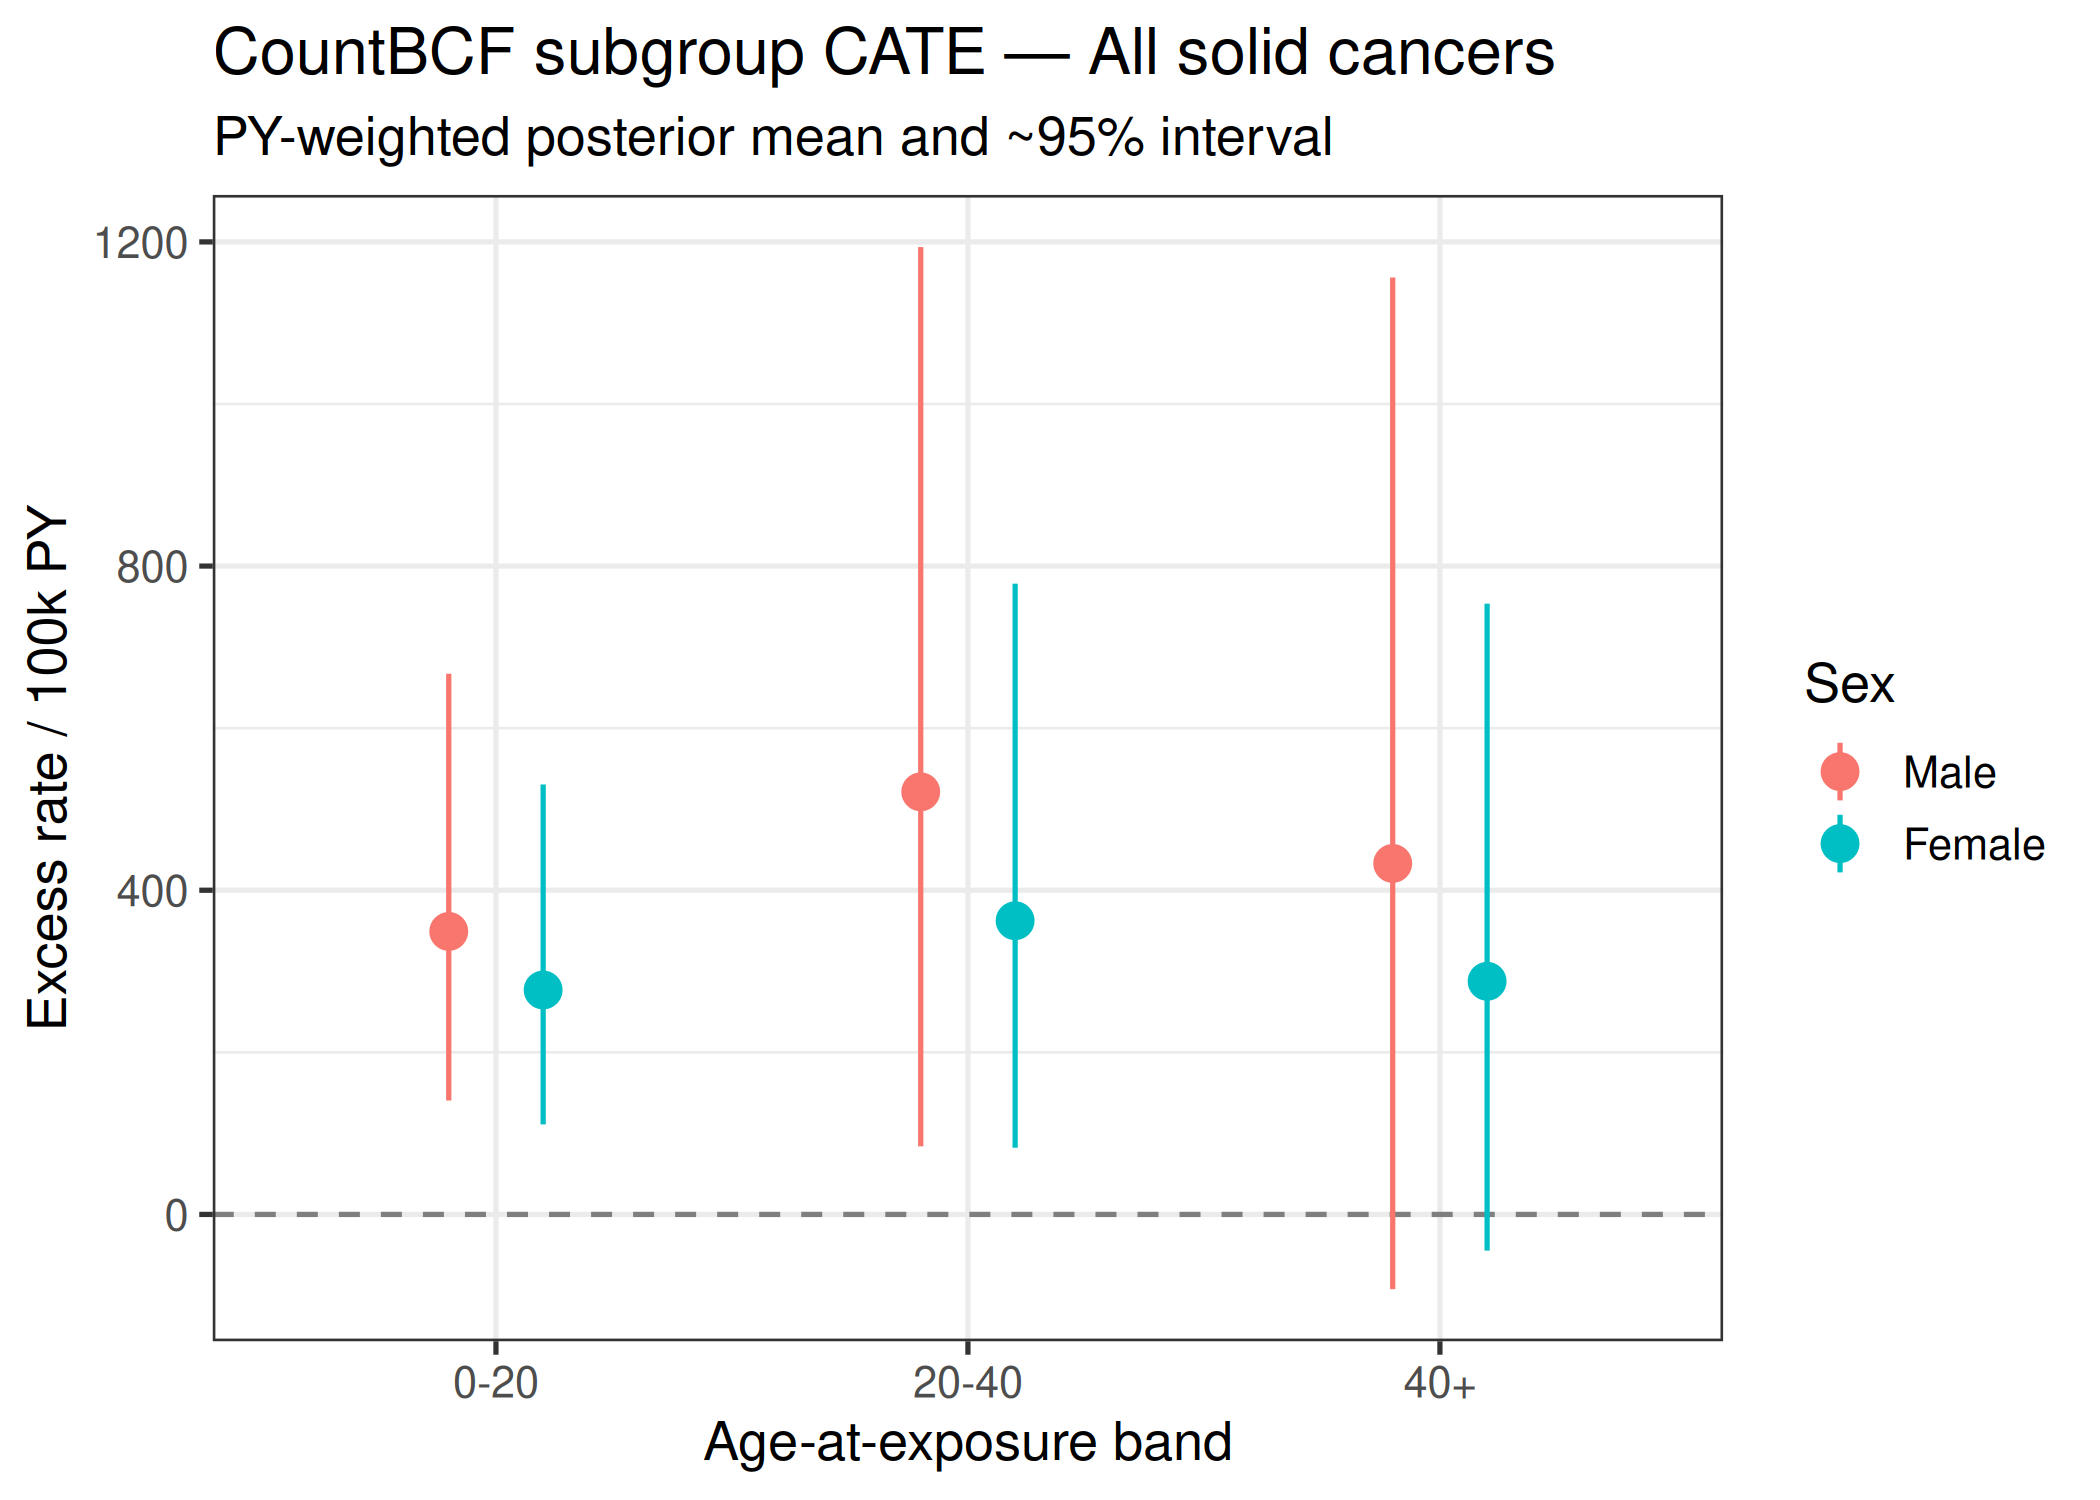
\includegraphics[width=\linewidth]{solid_cate_subgroups.png}
  \caption{All solid cancers}\label{fig:subgroups-solid}
\end{subfigure}
\hfill
\begin{subfigure}{0.49\textwidth}
  \centering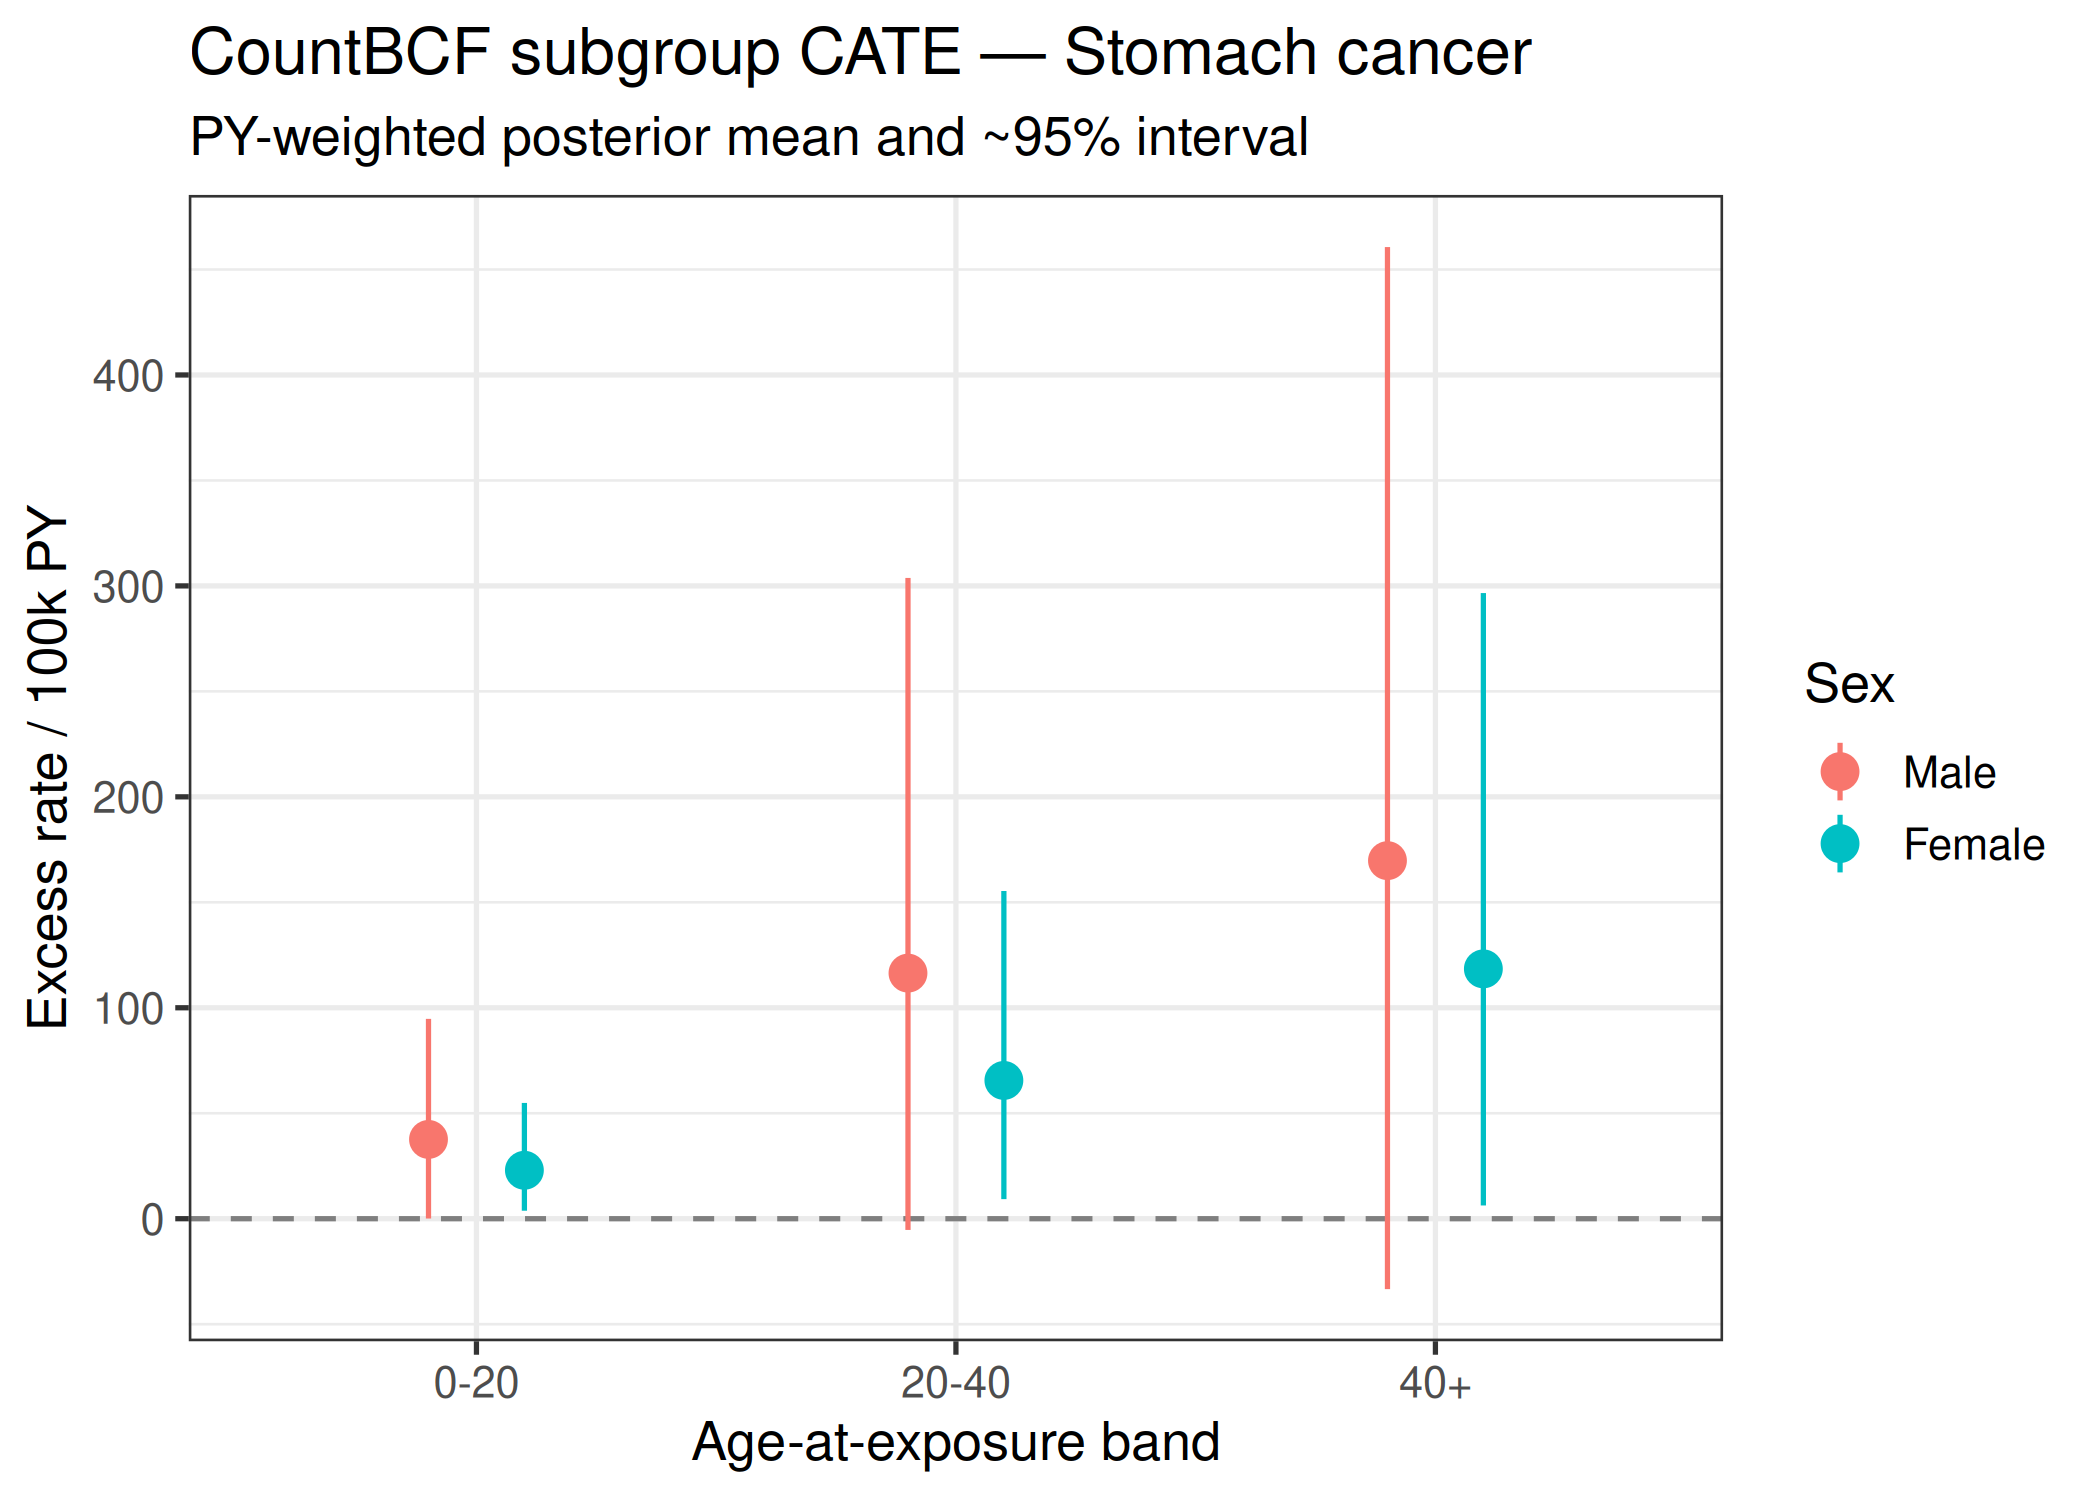
\includegraphics[width=\linewidth]{stomach_cate_subgroups.png}
  \caption{Stomach}\label{fig:subgroups-stomach}
\end{subfigure}
\caption{\textbf{Honest uncertainty that widens where the data thin out.}
Person-year-weighted posterior-mean subgroup CATE (excess cases$/10^5$~PY) for
the high-dose contrast with $\approx 95\%$ intervals, by age-at-exposure band
and sex. The intervals broaden sharply for the oldest-exposed ($40+$) band ---
the sparsest stratum --- and the solid-cancer female lower bound reaches zero,
exactly the region where the plateau/upturn of Figure~\ref{fig:err-agex} is
prior-dominated rather than data-driven.}
\label{fig:subgroups}
\end{figure}

A note on mechanism, offered as interpretation rather than as something the
data prove. The age-at-exposure ERR decline is consistent with a
``longer-fuse'' picture in which younger tissue has more remaining stem-cell
divisions for an initiated clone to expand \citep{icrp131}, while the plateau
at older ages is consistent with a shift from initiation-driven risk in the
young toward promotion of pre-existing pre-malignant clones in the old ---
a promotional channel that need not scale to zero \citep{shuryak2010}. The
shallow stomach age-at-exposure slope is consistent with gastric
carcinogenesis being governed by strong, later-acting non-radiogenic
promoters --- \emph{H.\ pylori}, dietary salt --- that dilute the
age-at-exposure radiation signal \citep{uemura2001}, and the female-higher
stomach ERR coexists comfortably with much higher male \emph{baseline}
stomach incidence, since a lower baseline inflates the relative scale
\citep{camargo2012}.

\subsection{Synthesis and caveats}
\label{sec:applied-synthesis}

Table~\ref{tab:applied-checklist} collects the convergence/divergence
verdicts. Of twelve testable claims, ten are convergent with the LSS canon on
shape, sign and ranking; one (the old-age-at-exposure ERR shape) is
convergent with a recognised contested position rather than the textbook
default; and exactly one (the solid-cancer sex ERR direction) genuinely
diverges in the primary specification --- and is explained by dose-surrogate
dilution of the female-driving sites together with the $2$~Gy / three-level
design, reversing to the canonical female-higher direction once the dose
range is widened (Table~\ref{tab:applied-sexsens}). CountBCF turned a
single ATE into a governed effect surface and read essentially the whole of
the established radiation-epidemiology structure out of $19{,}742$ cells,
with honest per-cell uncertainty that widens exactly where the data thin out,
\emph{without being told a single interaction term}.

\begin{table}[htbp]
\centering
\caption{Convergence/divergence checklist, CountBCF versus the canonical LSS
literature. Comparisons are on shape, sign and ranking, not magnitude.}
\label{tab:applied-checklist}
\small
\begin{tabular}{p{0.40\textwidth}p{0.29\textwidth}p{0.22\textwidth}}
\toprule
CountBCF result & Literature & Verdict \\
\midrule
Solid ERR falls $\sim$5$\times$ from age-at-exp.\ $<$10 to 40+ & Strong ERR decline with age at exposure \citep{preston2007,grant2017} & Convergent \\
Solid ERR plateaus $\approx 0.25$, faint upturn after $\sim$50 & Contested; plateau-after-30 / middle-age non-monotonicity, or aggregation artifact \citep{beirvii2006,shuryak2010,little2009} & Convergent with contested position \\
Solid EAR rises $\sim$7$\times$ with attained age & EAR rises with attained age (baseline-driven) \citep{preston2007,grant2017} & Convergent \\
EAR peaks at age-at-exp.\ 20--30 while ERR peaks youngest & Classic EAR-vs-ERR tension \citep{pierce2000} & Convergent \\
ERR flat over time since exposure; EAR rises & Persistent multiplicative excess \citep{preston2007,ozasa2012} & Convergent \\
Stomach female ERR $>$ male (0.46 vs 0.35) & Female stomach ERR higher \citep{sakata2019} & Convergent \\
Solid male ERR $\approx$/$>$ female (0.83 vs 0.76); reverses to female-higher under $\leq$4 Gy & Canonical: female all-solid ERR higher \citep{preston2007,grant2017} & \textbf{Divergent (primary spec)} --- design-driven (2 Gy cap/binning) $+$ dose-surrogate dilution \citep{walsh2016,brenner2018} \\
No Hiroshima--Nagasaki difference, either scale & DS02 reconciles the cities \citep{preston2007,ds02} & Convergent \\
Stomach age-at-exp.\ slope much shallower than solid & Stomach unmodified by age at exposure \citep{sakata2019} & Convergent \\
ERR scales $\sim$linearly, moderate vs.\ high & Approx.\ linear $\leq$2 Gy (curvature debated) \citep{preston2007,cologne2019} & Convergent (first order) \\
Moderate-dose stomach a coherent null (RR 1.04) & Low-dose attenuation, weakly radiogenic site \citep{sakata2019} & Convergent \\
Male EAR $>$ female, both sites & Male EAR higher for non-sex-specific sites \citep{preston2007} & Convergent \\
\bottomrule
\end{tabular}
\end{table}

Several caveats bound the interpretation. The aggregate endpoint is
colon-dose-anchored, so its site mixture is not the published all-solid
endpoint; this drives the sex divergence and means magnitudes are not
$1{:}1$ comparable with site-specific LSS tables. The person-year table is
cross-sectional, so one-dimensional covariate margins entangle age at
exposure with attained age --- the CATE \emph{surface}
(Figure~\ref{fig:heatmap}) is the unconfounded object, the margins are
projections. Sparse corners (oldest age at exposure,
extreme attained ages) are prior-dominated --- shrunk toward the positive
global mean effect --- and carry the widest intervals, so apparent features
there, such as the oldest-age-at-exposure upturn, should be read as
prior-driven rather than data-driven.
Survivors contribute person-years to multiple cells, so both the GLMs and
CountBCF treat as independent rows that are not fully independent; intervals
are therefore mildly optimistic, and a cluster random effect (which CountBCF
supports through \texttt{randeff\_design}) is the rigorous next step.
Finally, all effect modification here is \emph{discovered}, not imposed: no
age-at-exposure, attained-age, sex or city interaction was specified, so the
model can under-state heterogeneity in data-poor regions rather than
manufacture it --- which, for a method whose central claim is honest
uncertainty on the CATE, is the conservative and desirable failure mode.

A final caveat concerns the causes we could not measure. Individual smoking,
\emph{H.\ pylori} infection and dietary salt are absent from
\texttt{lssinc07.csv}, and they bear differently on the two estimands. Because
such exposures are approximately \emph{balanced} across dose bands --- dose was
assigned by location and shielding, not by lifestyle --- the \emph{ATE} is
only mildly susceptible to confounding from them, which is part of why the
GLM convergence of Section~\ref{sec:applied-ate} is believable. The E-values
make this concrete: explaining away the headline high-dose solid ATE (RR
$1.56$) would require an unmeasured confounder associated with \emph{both}
dose and incidence by a risk ratio of $\approx 2.5$ (point) or $\approx 2.1$
(confidence limit; Table~\ref{tab:applied-ate}) --- far beyond the reach of a
lifestyle factor like smoking, whose association with location-assigned dose
is near unity. The \emph{CATE} is more exposed: heterogeneity recovered at smoking- or
infection-related sites could in part reflect unmodelled
radiation$\times$smoking or radiation$\times$\emph{H.\ pylori} interaction
rather than pure effect modification by the demographic covariates. That
concern is strongest for stomach, where non-radiogenic promoters dominate the
background, and weak for colon and the solid aggregate. We therefore read the
ATE as well insulated, and the CATE surface as trustworthy where competing
causes are weak and provisional where they are strong; modelling these
interactions directly, as opposed to caveating them, would require the
individual smoking and infection covariates that the public person-year table
does not contain. More generally, the robustness checks reported here ---
the E-values of Table~\ref{tab:applied-ate} and the moderate-dose stomach null
that acts as a partial negative control --- serve to \emph{characterize} the
potential influence of unmeasured confounding on these conclusions, not to
eliminate it; identification still rests on the assumptions stated in
Section~\ref{sec:applied-design}.

% =====================================================================
% =====================  DROP-IN: END SECTION  ========================
% =====================================================================

\clearpage
\bibliographystyle{plainnat}
\bibliography{Applied_Study_Section}

\end{document}
